\documentclass[a4paper]{article}
% !TeX spellcheck = en_US 

%%%%%%%% CREATE DOCUMENT STRUCTURE %%%%%%%%
%% Language and font encodings
\usepackage[english]{babel}
\usepackage[utf8x]{inputenc}
\usepackage[T1]{fontenc}
\usepackage{eurosym}
%\usepackage{subfig}
\usepackage{listings}
\usepackage{siunitx}

\lstset{language=C++,
	basicstyle=\ttfamily,
	keywordstyle=\color{blue}\ttfamily,
	stringstyle=\color{red}\ttfamily,
	commentstyle=\color{green}\ttfamily,
	morecomment=[l][\color{magenta}]{\#}
}
%% Sets page size and margins
\usepackage[a4paper,top=3cm,bottom=2cm,left=2cm,right=2cm,marginparwidth=1.75cm]{geometry}
%% Useful packages
\usepackage{amsmath}
\usepackage{chngcntr}
\counterwithin{figure}{section}
\counterwithin{table}{section}
\usepackage{graphicx} 
\usepackage{multirow}
\usepackage{makecell}
\usepackage{tablefootnote}
\usepackage[colorinlistoftodos]{todonotes}
\usepackage[colorlinks=true, allcolors=black]{hyperref}
\usepackage{caption}
\usepackage{subcaption}
\usepackage{sectsty}
%\usepackage{apacite}
\usepackage{float}
\usepackage{titling} 
\usepackage{blindtext}
\usepackage{url}            % simple URL typesetting
%\usepackage[square,sort,comma,numbers]{natbib}
\usepackage[colorinlistoftodos]{todonotes}
\usepackage{xcolor}
%\usepackage[table,xcdraw]{xcolor}
\definecolor{darkgreen}{rgb}{0.0, 0.4, 0.0}
\usepackage{array}
\usepackage{pgfplots}

\counterwithin{figure}{section}
\counterwithin{table}{section}

\usepackage{pifont}% http://ctan.org/pkg/pifont
\newcommand{\cmark}{\ding{51}}%
\newcommand{\xmark}{\ding{55}}%

\usepackage[acronym]{glossaries}
\makenoidxglossaries

\renewcommand*{\glstextformat}[1]{\textcolor{black}{#1}}
\glsdisablehyper
\newacronym[plural=AVs]{AV}{AV}{Autonomous Vehicle}
\newacronym[plural=VRUs]{VRU}{VRU}{Vulnerable Road User}
\newacronym[plural=OGMs]{OGM}{OGM}{Occupancy Grid Map}
\newacronym{DST}{DST}{Dempster-Shafer Theory}
\newacronym{BEV}{BEV}{bird's-eye view}
\newacronym{FOD}{FOD}{Frame of Discernment}
\newacronym{BBA}{BBA}{Basic Belief Assignment}
\newacronym{NN}{NN}{Artificial Neural Network}
\newacronym{STIP}{STIP}{Stanford-TRI Intent Prediction}
\newacronym{ECP2.5D}{ECP2.5D}{Eurocity Persons 2.5D}
\newacronym{BDD100K}{BDD100K}{Berkely DeepDrive 100K}
\newacronym{KITTI}{KITTI}{Karlsruhe Institute of Technology and Toyota Technological Institute}
\newacronym{MSE}{MSE}{Mean Squared Error}
\newacronym{MeSE}{MeSE}{Median Squared Error}
\newacronym{SSIM}{SSIM}{Structural Similarity Index Measure}
\newacronym{IS}{IS}{Image Similarity}
\newacronym{TPR}{TPR}{True Positive Rate}
\newacronym{TNR}{TNR}{True Negative Rate}
\newacronym{FPR}{FPR}{False Positive Rate}
\newacronym{PPV}{PPV}{Positive Predictive Value}
\newacronym{ROC}{ROC}{Receiver Operating Characteristic}
\newacronym{ConvLSTM}{ConvLSTM}{Convolutional Long Short-Term Memory}
\newacronym{CNN}{CNN}{Convolutional Neural Network}
\newacronym{RNN}{RNN}{Recurrent Neural Network}
\newacronym{LSTM}{LSTM}{Long Short-Term Memory}
\newacronym{DOGMa}{DOGMa}{Dynamic Occupancy Grid Map}
\newacronym{AAConvLSTM}{AAConvLSTM}{Attention Augmented \gls{ConvLSTM}}
\newacronym{GRU}{GRU}{Gated Recurrent Unit}
\newacronym{STM}{STM}{Spatial Transformer}
\newacronym{MFE}{MFE}{Motion-Flow Extraction}
\newacronym{STC}{STC}{Spatio-Temporal Convolution}


\newcommand{\airquote}[1]{``#1''}

\usepackage{booktabs}
\newenvironment{conditions}
{\par\vspace{\abovedisplayskip}\noindent\begin{tabular}{>{$}l<{$} @{${}={}$} l}}
	{\end{tabular}\par\vspace{\belowdisplayskip}}
\setlength{\parindent}{0in} 

\usepackage{pdflscape}
\usepackage{afterpage}

%%%%%%%% DOCUMENT %%%%%%%%
\title{Literature Review on Traffic Scene Motion Prediction using Occupancy Grid Maps}
\author{Rutger Dirks}
\date{\today{}}


\begin{document}
	\fontfamily{ptm}\selectfont % Fonts: qcr, lmodern(lmr), mathptmx(ptm)
	
	%%%% Title Page
	\begin{titlepage}

		\maketitle{}
		
		\begin{figure}[h]
			\centering
			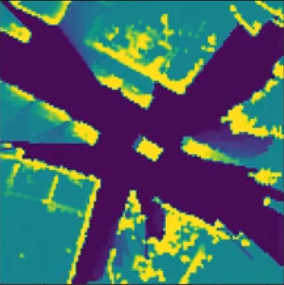
\includegraphics[width=0.6\linewidth]{Figures/Title_Page_OGM}
			\label{fig:title_page}
		\end{figure}
		
		\begin{center}
			% Department
			\textsc{3mE Department of Cognitive Robotics - Intelligent Vehicles}\\[1cm]
			% University
			\textsc{\LARGE Delft University of Technology}\\[1cm]
			%Supervisors
			\textsc{Supervisors: Ewoud Pool, Hidde Boekema, and Dariu Gavrila}\\[5cm]
		\end{center}


		

	\end{titlepage}
	\fontfamily{ptm} \selectfont	
	\newpage
	\printnoidxglossary[type=acronym]
	\printacronyms
	\newpage
	\tableofcontents{}	
	\newpage	
	\section{Introduction} \label{sec:intro}
% Introduction
In 2017, the European Union counted around $25300$ fatalities on the EU roads, of which 46\% were vulnerable road users (e.g. pedestrians and (motor-)cyclists). Although the EU roads account for the safest roads in the world, the number of road fatalities have stagnated in the past few years. At this rate, the EU's goal of reaching fewer than $16000$ fatalities in 2020 could not be achieved. Especially vulnerable road user fatalities have not decreased at the same pace as the overall population. Any progress to increase the safety of vulnerable road users will have a significant impact to the road fatality rate. \cite{vademecumeu2018road} \\

\glspl{AV} are expected to increase road safety because the autonomy would erase the effects of human error \cite{cui2019review}, since more than 90\% of the accidents is caused by human error \cite{eu2020website}. However, \glspl{AV} are not yet safe enough to deploy on the roads and still a lot of research should be done before fully autonomous vehicles can be introduced to the market \cite{okuda2014survey} \cite{cui2019review}. \\

One of the current challenges to autonomous driving is to capture road user intent and to make accurate real-time trajectory predictions of other road users \cite{ohn2016looking}. Especially predicting the behavior of \glspl{VRU} is important \cite{ohn2016looking} \cite{cara2015classification} because good anticipation of a \gls{VRU}'s behaviour results in faster reactions and thus can prevent more accidents \cite{djuric2020uncertainty}. Predicting \gls{VRU} behavior is additionally challenging compared to predicting other (motorized) road users, because the motion patterns of \glspl{VRU} are complex and mutable depending on the static and dynamic obstacles they encounter \cite{chou2020predicting}. Therefore, a motion prediction method is needed that can also accurately predict the motion of \glspl{VRU}.\\

Currently, there are some promising methods to predict the motion of the entire \gls{AV}'s environment (including \glspl{VRU}). These methods make use of an \glsfirst{OGM} to capture the \gls{AV}'s environmental context. An \gls{OGM} is a rasterized \gls{BEV} map corresponding to the \gls{AV}'s environment that contains occupancy information in each grid cell of the raster. Given the \gls{AV}'s environmental sensor data (e.g. from a LiDAR, camera, or radar), each grid cell's state in the \gls{OGM} is updated to a new occupancy value (Empty, Occupied, or Uncertain). Deep learning can be used to predict future \glspl{OGM} sequences of an \gls{AV}'s environment, given past \gls{OGM} sequences. Since an \gls{OGM}'s form is similar to an image - a matrix containing values between 0 (Empty) and 1 (Occupied) - convolutional neural networks can be used to efficiently extract useful features from it \cite{albawi2017understanding}. Then, a sequential neural network can be used to process a sequence of the extracted features to capture the past states and behavior of the \gls{AV}'s environment. The information of the past is then used by the neural network to generate \gls{OGM} predictions that describe the future environment of the \gls{AV}. \\

%TODO: IMage of the OGM from the title page

This literature study gives an overview of what the current research areas and challenges for the future are regarding motion prediction using \glspl{OGM}. The conclusion of this study forms the basis for the Master thesis research proposal at the end of this literature review. \\

In the following sections of this introduction, first, the problem of motion prediction is described. Then, current solutions to motion prediction challenges and their limitations are briefly discussed. After discussing the challenges and limitations of current solutions, it is explained why \gls{OGM} prediction methods are a promising all-encompassing solution to those current challenges. Then, one main research question and four sub-questions are posed to investigate the stated motion prediction problem regarding \gls{OGM} prediction methods. The following chapters provide information from literature to answer the main and sub-questions posed in this introduction. This chapter ends with a short overview of the content of each chapter.

\subsection{Problem Description} 
%Problem
The problem of motion prediction is an inferencing task. Based on evidence in the form of current and/or past observations and experience, future states (trajectories) of one or more actors (i.e. traffic participants such as cars, cyclists, and \glspl{VRU}) must be predicted for a pre-determined time horizon, within a certain accuracy and certainty, which needs to be executed within a specific time limit. This problem statement will be explained more elaborately in these following paragraphs. \\

Actors, in this problem statement, are traffic participants including, but not limited to, cars, riders, cyclists and pedestrians (\glspl{VRU}). \\

The evidence that supports the actor's predictions can have the form of current and/or past observations, and obtainable experience. The current and past observations are sensor data acquired from the environment (observations) by either static observers (the sensors are static and record the environment) or dynamic observers (the sensors move within the environment while recording it) or both.
Then, obtainable experience are generalizations of traffic, including traffic behavior and traffic environments (experience). These generalizations can be based on statistics, they can be based on assumptions, and they can be learned using historic observations. \\

Based on the investigated literature, the future states can be represented as one of the three following forms in the predictions. 

\begin{enumerate}
	\item The predictions are estimated future state values of an actor's centroid, including its coordinates and sometimes orientations, which are projected into the environment representation.
	\item The predictions are estimations of the future actor's representation within the current environment representation.
	\item The predictions are estimations of the entire future environment representation.
\end{enumerate}

\begin{figure}[h!]
	\centering
	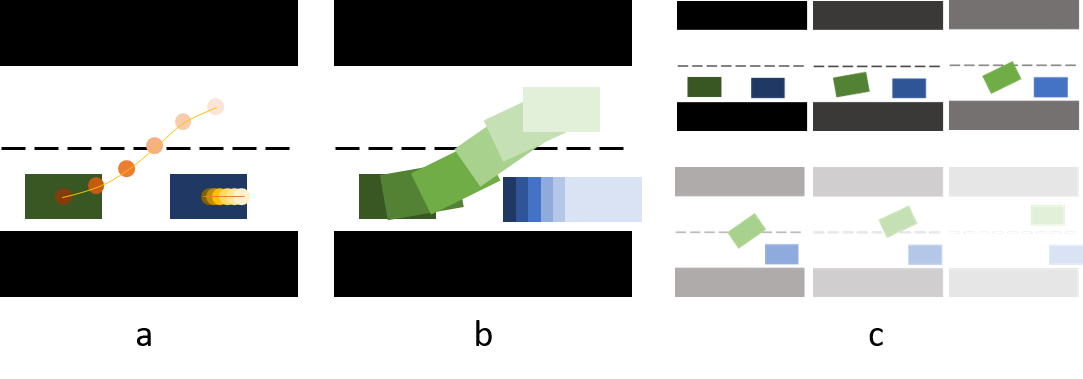
\includegraphics[width=0.8\linewidth]{Figures/Introduction/Prediction_forms}
	\caption{This image shows the three prediction forms encountered in the literature. The black and white parts represent a road. The green and blue squares are representations of vehicles. The predictions are shown using a more fading color the further the prediction goes into the future. Figure a shows the prediction of future centroids projected into the environment representation. Figure b shows the prediction of future actor representations within the environment (the complete vehicles are predicted instead of the centroids only). Figure c shows the prediction of the entire future environment. In this case, also a prediction of the environment (road) is provided.}  
	\label{fig:pred_froms}
\end{figure}

Finally, the problem statement mentions a time horizon, that the predictions must be within a certain accuracy and certainty, and that it needs to be executed within a specific time limit. The time horizon is the amount of time into the future that the prediction must span. Ideally, the time horizon, the accuracy, the certainty, and the execution time of the predictions should be infinitely, exact, complete, and instantaneous, respectively. However, this is not possible in practice. Therefore, I think a suitable prediction method should predict further into the future, be more accurate, have more certainty, and be faster than a human can perform the task. Within the context of \glspl{AV}, this is a reasonable requirement in order for the \gls{AV} to be able to perform safer than humans can.   


\subsection{Current Solutions}
Over the past decade, much research has been done to find methods that solve the previously mentioned motion prediction problem. Table \ref{tab:overview_mot_pred} in Appendix \ref{app:appendixA} shows an overview of recent motion prediction papers and their respective methods. It is notable that most methods use a form of deep learning to predict trajectories in any of the forms as described in the problem description. What is also striking, is that relatively few papers have performed research which includes \glspl{VRU} in which the observer is dynamic (from a vehicle's point of view). Still, it is important that \gls{VRU} behavior prediction is investigated. \gls{VRU} collisions are likely to be fatal which makes accurate and early motion prediction necessary in order to respond safely to their actions \cite{rehder2018pedestrian}, \cite{chou2020predicting}, \cite{uah2020d4}. Therefore, \gls{VRU} behavior prediction is a relevant research topic regarding \glspl{AV}.\\
A major challenge in this research area is to predict \gls{VRU} motion for the long term. However, research on this topic faces a multitude of challenges. Accurate long-term predictions require the incorporation of environmental and social context. Moreover, implementing uncertainty and multimodality of the predictions and making the predictions fast enough for real-time applications in \glspl{AV} are also challenges that need to be solved. These major challenges and recent research to find solutions are described in the following subsections. 

\subsubsection{Long-term motion prediction}
For motion prediction, a prediction for which the prediction time horizon is more than 2 seconds is considered long-term \cite{hormann2020long}. Compared to other road users, \glspl{VRU} are highly maneuverable which makes it challenging to predict their behavior, especially for the long-term \cite{xiong2019recurrent}, \cite{rehder2018pedestrian}, \cite{rehder2018pedestrian}. Most prediction models assume that \gls{VRU} behavior is intention-driven and that those intentions can be inferred from certain cues, other than dynamics \cite{rehder2018pedestrian}. Therefore, detecting cues related to \gls{VRU} behavioral changes is important for achieving accurate long-term predictions \cite{pool2017using}. These cues can be related to the \gls{VRU}'s environment (e.g. traffic lights, zebra's, obstacles) or to the \gls{VRU}'s social interactions (e.g. evasion of other \gls{VRU}'s, distancing due to social norms, nearing another \gls{VRU}). The following two paragraphs elaborate on the incorporation of environmental and, respectively, social context in prediction models. Besides using cues to predict \gls{VRU}'s behavior, implementing the uncertainty of the predictions and incorporating multimodality is also researched, as well as making the models fast enough so that they can be implemented real-time on \glspl{AV}. These topics are also discussed below. 

\subsubsection{Environmental context}
Environmental context consists of the static and dynamic obstacles and semantic meaning within an actor's surroundings. Research suggested to incorporate environmental context because an actor's trajectory is highly influenced by its environment. Scene context can constrain the actor in its planned motions \cite{chou2020predicting}, \cite{pfeiffer2018data}, \cite{sadeghian2019sophie}, \cite{manh2018scene}. Especially to anticipate critical situations, taking into account the environmental context is expected to increase the prediction accuracy \cite{uah2020d4}. An example of how the use of traffic light information influences the predictions is shown in figure \ref{fig:env_cont}. The challenge is how to model that environmental context so that it is semantically representative, highly discriminative and generalizable to a variety of complex scenes. This way, it can be used as evidence to enable inferences about an actor's future trajectory \cite{varshneya2017human}. \cite{pool2017using} Shows that leveraging prior knowledge about an actor's environment can improve the trajectory predictions. Therefore, they suggest to extend the incorporation of environmental context even more with the expectation that it will further increase the prediction accuracy.  

\begin{figure}[h!]
	\centering
	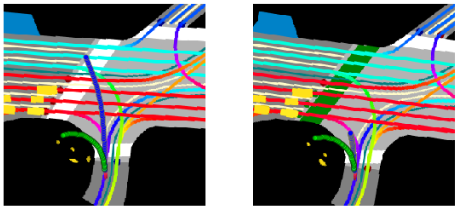
\includegraphics[width=0.5\linewidth]{Figures/Introduction/Environmental_Context_TRaffic_Light_Chou}
	\caption{This image shows an example of how the environmental context can be used to influence the predictions. On the left, the prediction (the blue trajectory) of the bicyclist (red) is shown when the traffic light in the scene is green. On the right, the bicyclist's prediction is shown when the traffic light turned red. The green trajectory is the ground truth. \cite{chou2020predicting}}  
	\label{fig:env_cont}
\end{figure}


\subsubsection{Social Context}
Social context consists of the static and dynamic actors, their semantic meaning, and their interactions within an actor's surroundings. When an actor navigates, it constantly tries to anticipate movements of surrounding actors to envision more than one feasible path it could take in order to adjust its own path and maneuver past or aside those surrounding actors \cite{sadeghian2019sophie}, \cite{manh2018scene}. Figure \ref{fig:soc_cont} shows how \cite{sadeghian2019sophie}'s prediction method takes into account social context. Therefore, one of the main factors that influence an actor's behavior is the its social context. It is expected that by incorporating social context into prediction models, the accuracy will increase significantly \cite{pfeiffer2018data}. 
Especially for pedestrian behavior, the social and environmental context is expected to be the leading evidence for predicting their behavior because pedestrians \airquote{are not expected to use any active forms of communication when interacting with vehicles and other road users} \cite{uah2020d4}. 

\begin{figure}[h!]
	\centering
	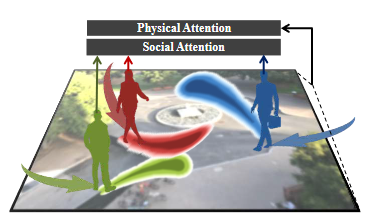
\includegraphics[width=0.4\linewidth]{Figures/Introduction/Social_context_Sadeghian}
	\caption{This image shows a schematic of how \cite{sadeghian2019sophie} uses the social context, and the scene context, to predict the behavior of the pedestrians (the green, red, and blue surfaces). The pedestrians are predicted to avoid each other while continuing in the general direction they walked in the past (the arrows). \cite{sadeghian2019sophie}'s method predicts physically and socially plausible trajectories.}  
	\label{fig:soc_cont}
\end{figure}

\subsubsection{Uncertainty and Multi-modality}
For the safety of AVs, uncertainty estimations for predictions are critical \cite{djuric2020uncertainty}. If an AV is aware of the confidence of its predictions, it can adjust its planned course to minimize the risk of collisions \cite{huang2019uncertainty}. For example, if an AV predicts that a pedestrian will not cross the road, but the confidence of that prediction is very low, the AV can adjust its course by leaving more room for the pedestrian in case the prediction is false. Without knowing the confidence of a prediction, such risk-avoiding course adjustments cannot be made. Besides including uncertainty estimations, it is important that predictions are multimodal. VRU behaviour is inherently multimodal because they easily change their course which is highly dependent on their environment \cite{cui2019multimodal}, \cite{tang2019multiple}. Incorporating multimodality is a challenge, because it requires good probability estimations and knowledge of the different modes. It either requires explicit labeling of the modes prior to training \cite{tang2019multiple}, or the modes could be learned. Because probability estimations are needed to make multimodal predictions, these methods are often researched together. \\

\cite{keller2013will} compares four different multimodal prediction models related to Bayesian principles. These models return the probability of stopping (whether a nearing pedestrian will stop, instead of cross the road). However, only two motion modes are considered in this research. \cite{pool2017using} Uses a Mixture of Linear Dynamical Systems to predict the probabilities of a cyclists going in one of the five pre-determined direction modes. This model also takes into account information about the road topology to enhance the predictions. The downside of these Bayesian models is that the computation time increases when more modes are added and when more context information is incorporated in the predictions. Moreover, adding more modes is a challenges in complex environments in which it is unclear what directions an actor can go to. Therefore, deep learning models are devised that can include multimodality in the predictions by learning the modes in a latent space and incorporating learned features of the VRU's context. \\
\cite{rehder2018pedestrian}, \cite{cui2019multimodal}, \cite{brito2020social} investigated deep learning models that, respectively, predict multimodal trajectories by training a network to learn the parameters of a Mixture Density Network that predicts multiple trajectories, train a network to choose the best of M hypothetical trajectory modes, and train a variational RNN that learns a conditional distribution of available modes from which the output Gaussian Mixture Model can be sampled. Although these methods all provide probabilities for the different available trajectory modes, still they do not provide a confidence estimation the model has about the multimodal predictions. \cite{huang2019uncertainty}'s research adds a confidence estimator to their multimodal prediction method that estimates the confidence of multiple predictors (See figure \ref{fig:multimod}). The predictor with the highest confidence value is considered for the trajectory prediction. 

\begin{figure}[h!]
	\centering
	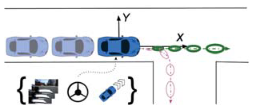
\includegraphics[width=0.4\linewidth]{Figures/Introduction/Multimodality_Huang}
	\caption{This image shows a schematic of how multimodal predictions can be made, given a past trajectory. Since the road allows for two directions the vehicle can move in, two predictions are made. One prediction in green, going straight. The other in red, going to the right. The prediction that goes straight forward is given the highest confidence value (thick green), which means that that trajectory is considered for the prediction.  \cite{huang2019uncertainty}}  
	\label{fig:multimod}
\end{figure}

\subsubsection{Real-time motion prediction}
Fast real-time computation is important in order to implement the prediction model on AVs. 
\cite{djuric2020uncertainty} Addresses the importance of real-time execution of prediction models. They state that certain prediction methods (e.g. Bayesian Networks and Inverse Reinforcement Learning) are inefficient and thus not feasible for real-time applications such as AVs. Therefore, it is important that the prediction methods are efficient enough so they can be applied online in AVs to increase VRU safety. Their method of using a CNN to predict future trajectories was succesfully tested real-time in an AV. However, this method only predicts future trajectories of vehicles, not VRUs. \\
\cite{brito2020social} stresses the importance for real-time predictions for applications in AVs as well. They developed the Social-VRNN that takes samples from a variational RNN's conditional distribution to predict pedestrian trajectories. Previous research used other methods, such as Generative Adversarial Networks (GANs), which required more samples for accurate predictions compared to the Social-VRNN, making the Social-VRNN much faster. However, this method does not yet perform in real-time.  \\
\cite{chou2020predicting} aims for the most efficient motion prediction models without it affecting the accuracy because it "is necessary to achieve real-time inference onboard an SDV in crowded urban environments comprising large number of VRUs" \cite{chou2020predicting}. Without real-time online motion prediction, AVs cannot make use of these methods and the safety of VRUs will not improve. They developed a real-time motion prediction method, using a CNN, for all road users. Their solution shows promising results, but the dataset requires more VRU data to match the state-of-the-art prediction accuracy. 

\subsubsection{The promising solution}
The state-of-the-art research in the previous paragraphs show that Deep Learning methods provide means to include environmental and social context, as well as uncertainty information, to make better, long-term, path predictions including those of \glspl{VRU}. Several Deep Learning methods use \glspl{OGM}, a grid-based representation of the environment obtained from sensors on \glspl{AV}, as input data to predict future \glspl{OGM} for the long-term. \glspl{OGM} contain occupancy data of the \gls{AV}'s environment which is often extended with uncertainty information of the occupied areas. Furthermore, the \gls{OGM} can be extended with additional information layers such as semantics and dynamics of the occupied regions. Correlations of the environment and its actors can be captured when the \gls{OGM} is processed by a convolutional neural network. Predicting \glspl{OGM} is expected to be more accurate, also for long-term predictions, due to the amount of information that can be stored in the OGM. Attempts to make real-time \gls{OGM} predictions are succeeding (Mohajerin \cite{mohajerin2019multi} shows that it can take 60ms to predict \glspl{OGM} 1s into the future), making these methods, using \glspl{OGM} as environment representation, a promising one for motion prediction research. All in all, the motion prediction methods that use \glspl{OGM} can provide solution to all challenges stated in the previous paragraphs. That is why \gls{OGM} prediction is a promising solution that is worth investigating, which leads to the following section about this literature reviews research questions. \\


\subsection{Research Questions}
Because of the potential of \glspl{OGM}, this literature review focuses on the prediction of \glspl{OGM} using Deep Learning. Currently, state-of-the-art research regarding motion prediction in traffic scenes makes use of \glspl{OGM}. To give an overview of these \gls{OGM} prediction methods and to find out which method provides the best predicitons, the following main research question is asked: \textit{"What is the best method to perform traffic scene \gls{OGM} prediction using Deep Learning?"} \\

In this review, several sub-questions are asked in order to answer the main question. The reasoning behind the sub-questions, followed by the sub-questions is described below. \\ 

First, it is important to know what an \gls{OGM} is and how they can be generated from an \gls{AV}'s sensor data. Research shows that \glspl{OGM} can be generated using several methods \cite{collins2007occupancy} \cite{ribo2001comparison} \cite{thrun2003learning}. Besides several generation methods that compute occupancy information for each \gls{OGM}'s grid cell, the \glspl{OGM} can also be extended with other information such as semantics \cite{lu2019monocular}, dynamics \cite{nuss2018random}, and 3D information \cite{degerman20163d}. Combinations of the different generation methods and data extensions will result in different \gls{OGM} forms. This leads to the first sub-question: \textit{What \gls{OGM} form is most suitable to use in \gls{OGM} prediction methods?} \\

Second, to generate the \glspl{OGM}, a dataset should be used that contains sequences of traffic scene sensor data from an \gls{AV}'s point of view. It is important that occupancy information can be extracted from the data. Additionally, it is a perk if the datasets also contains 3D, semantic, or dynamic information about the traffic scenes for the extended \gls{OGM} forms. There exist several datasets (view table \ref{tab:datasets_overview}) that contain this kind of data. To find out which of these datasets is the best to use for \gls{OGM} generation and prediction, the second sub-question is asked: \textit{What dataset is most suitable to generate OGM sequences for OGM prediction?} \\

Third, to determine which \gls{OGM} prediction method performs best, the quality of the \gls{OGM} predictions need to be evaluated per method so the different methods can be compared. When evaluating, the \gls{OGM} predictions will be compared to the ground truth \glspl{OGM}. The more the predictions are similar to the ground truth, the better that prediction method performs. Evaluation can be done by visually comparing the predictions to ground truth \glspl{OGM} \cite{ribo2001comparison}. However, this evaluation method is subjective and thus can result in unreliable performance scores. Therefore, \cite{collins2007occupancy} summarizes some quantitative evaluation methods that use image similarity principles to evaluate \glspl{OGM}. Quantitative metrics can provide an objective means for performance evaluation. However, each metric measures a different aspect of the \gls{OGM}. It is therefore important that a metric is chosen that best evaluates the similarity accuracy between \glspl{OGM}. This leads to the third sub-question: \textit{What is the best quantitative metric to determine the accuracy of a predicted OGM?} \\

Fourth, there are several state-of-the-art deep learning methods that perform \gls{OGM} prediction. To find out which of those methods are the best ones, they must be evaluated and compared with each other. To answer the main questions, this fourth sub-question is asked: \textit{What Deep Learning method generates the best OGM predictions?}

\subsection{Chapter overview}
The posed research questions will be answered in the following chapters of this literature review. Chapter \ref{sec:ogm} provides information about \glspl{OGM} and answers the first sub-question. In chapter \ref{sec:datasets}, criteria are set which an ideal dataset should meet to use it for \gls{OGM} prediction. This chapter will answer the second sub-question. The third sub-question will be answered in chapter \ref{sec:metrics}, in which several metrics to determine the quality of \glspl{OGM} are compared according to some criteria that are required for accurate and safe (related to \gls{AV}'s) error estimations of \gls{OGM} predictions. The fourth sub-question will be answered in chapter \ref{sec:ogm_methods}, in which an overview of \gls{OGM} prediction methods using deep learning is provided. Chapter \ref{sec:conclusion} contains a conclusion in which the main research question of this literature review is answered. Then, chapter \ref{sec:future} discusses some topics for future work that result from this literature study. The final chapter is a research proposal for my Master thesis to which the conclusion of this literature review provides the basis.



%% After the Challenges: Each challenge becomes a topic/section
%% Long term motion prediction: discuss most used methods up until deep learning methods
%% Discuss how later the incorporation of environment, social, uncertainty/mutlimodality was also incorporated
%% And what methods are used for that
%% Dicuss Why real-time motion prediction is important and what the fastest computation times are for each other challenge
%% And how faster methods can be researched 
%%

%%% NEW LIT PART

%% Before, the main challenges to motion prediction are described. Then, ... thought of using OGMs to predict the future because in an OGM env and social context can be incorporated, multimodal paths and uncertainty can be computed, and some prediction methods can even perform real-time. But what are the advantages and disadvantages? Is it really better?




	\newpage
	\section{Occupancy Grid Mapping} \label{sec:ogm}
In 1985 Moravec and Elfes \cite{moravec1985high} investigated the use of sonar measurements to map the surroundings of a robot. By gathering sonar measurements from multiple points of view (having several sensors on the robot) and from multiple instances in time, information about the robot's surroundings is accumulated. This information is used to compute the state of each cell within a rasterized 2D \gls{BEV} map of the robot's surroundings is 'occupied', 'unoccupied', or 'unknown' (when there is no sensor data available of that cell), as can be seen in Figure \ref{fig:OGMBEVmoravec}. This is an example of environment representation called an \glsfirst{OGM}. \\

\begin{figure}[h]
	\centering
	\includegraphics[width=0.6\linewidth]{Figures/Occupancy_Grid_Map/The_Two-dimensional_Sonar_map}
	\caption{This image shows an \gls{OGM} of a robot's surrounding environment. The solid lines represent the outline of the room and of the major objects that formed the robot's environment. The large circles in the image are the positions at which the robot performed measurements of its surroundings. The measurements are used to generate the \gls{OGM}, which is a \gls{BEV} raster in which each cell represents the state of an area within the environment. Each cell contains a symbol or white space. Empty areas with a high certainty factor are represented by white space. Empty areas with lower certainty factors are represented by "+" symbols of increasing thickness the lower the certainty. Occupied areas are represented by "x" symbols, and Unknown areas by "." symbols. Image from \cite{moravec1985high}.}
	\label{fig:OGMBEVmoravec}
\end{figure}

Formally, the \gls{OGM} is often represented in a tensor or matrix, $m$, of which each element (cell), $m_{i,j}: i \in [0, M],j \in [0, N]$, represents the occupancy state of an area in the robot's surrounding world. The size of that area depends on the sensor's and grid cell's resolution. The occupancy probability of a cell $m_{i,j}$ is a discrete random variable with two exclusive and exhaustive values, occupied ($O$) and empty ($E$), resulting in equation \ref{eqn:occ_empt} \cite{elfes1989using}. Therefore, knowing only the probability of a cell being occupied $P[m_{i,j} = O]$, which is a number between $0$ and $1$, is enough to determine a cell's state. Given a cell's probability of being occupied, one out of three different states is assigned to that cell based on its probability value. If the probability value is close to $0$, the state is 'Empty', while with a probability value close to $1$ the state is 'Occupied'. If a cell's probability of being occupied is $0.5$, which means that the probability of the cell being empty is also $0.5$, it will be assigned the 'Unknown' state. This is the case for cells corresponding to areas that are unobserved or areas of which conflicting measurements are obtained. \\

\begin{equation} \label{eqn:occ_empt}
	P[m_{i,j} = O] + P[m_{i,j} = E] = 1
\end{equation} 

\hfill \break

For simplicity, the notation $m_{i,j}$ will be used for the case where the cell is occupied $m_{i,j} = O$ and $\neg m_{i,j}$ for the empty state $m_{i,j} = E$.
These state values can be determined in several ways. In section \ref{subsec:prob_OGM}, two probabilistic methods to obtain occupancy state values and generate \glspl{OGM} will be discussed. The first method uses an inverse sensor model and the second uses a forward sensor model. In section \ref{subsec:evid_OGM}, an evidential method for \gls{OGM} generation that uses the \gls{DST} will be discussed. Then, in section \ref{subsec:alt_OGM}, some alternative, less common \gls{OGM} generation methods are briefly discussed.
Besides ways to generate the traditional \gls{OGM} maps that provides information about the cell occupancy, there are extended \gls{OGM} forms that contain more information. Section \ref{subsec:OGM_ext_form} will elaborate on some of those extended forms. Finally, section \ref{subsec:OGM_conclude} concludes this chapter by answering the question: \airquote{\textit{What \gls{OGM} form is most suitable to use in \gls{OGM} prediction methods?}}

%Sources: Environment Perception Using Grid Occupancy, Fusion-2014, using occupancy grids for mobile robot.., probabilistic algorithms in robotics, Learning Occupancy Grids With Forward Sensor Models, Comparative Study of Inverse and Forward Sensor Models


\subsection{Probabilistic Occupancy Grid Mapping} \label{subsec:prob_OGM}
In probabilistic occupancy grid mapping, Bayesian reasoning is used to estimate the state of each cell in the grid. Two processing stages are required to compute the probability of the cell states. First, a sensor measurement is interpreted using a sensor model. Second, the sensor reading is used to update the \gls{OGM} cell's estimates using Bayes' theorem. \cite{elfes1990occupancy} \cite{moras2014evidential}. The two main sensor models that are used to interpret the sensor data are the inverse sensor model \cite{elfes1990occupancy} and the forward sensor model \cite{thrun2003learning}. The selected sensor model affects the assumptions that can be made about the \gls{OGM} and thus affects the performance and computing time of the updated \gls{OGM} cell states. Both sensor models and their implementation of the two processing stages, using Bayes' theorem, will be explained in the next two subsections. In the third subsection, both models will be compared. 

\subsubsection{Bayesian update with inverse sensor model}
The inverse sensor model is formulated according to formula \ref{eqn:inv_sens_dep}. It signifies the conditional probability of the complete occupancy grid map of the environment $m$, given the complete sets of sensor measurements $z_{1:T}$ and corresponding robot poses $x_{1:T}$. This model obtains the map state probability inversely to how the measurements are generated, since measurements are generated \textit{given} the map (environment). \cite{carvalho2013comparative}. 

\begin{equation} \label{eqn:inv_sens_dep}
	p(m|z_{1:T},x_{1:T})
\end{equation}

Given an \gls{OGM}'s size of $M\times N$, there are $2^{M\times N}$ possible grid configurations. As a result, the required computing power needed to estimate a complete \gls{OGM} scales exponentially with the grid size. To tackle this, each cell in the \gls{OGM} is assumed to be conditionally independent given the measurements and the poses, which results in equation \ref{eqn:inv_sens_indep}, where $m_{i,j}$ stands for a single grid cell's occupied state. This computation requires much less computing power. \cite{UoP2021} \cite{carvalho2013comparative}.

\begin{equation} \label{eqn:inv_sens_indep}
	p(m|z_{1:T},x_{1:T}) = \prod_{i,j}^{} p(m_{i,j}|z_{1:T},x_{1:T}) 
\end{equation} 

Also, a static world assumption is made in equation \ref{eqn:inv_static_assum1} which means that a measurement $z$ at time $t$ is conditionally independent from the previous measurements and poses, given the \gls{OGM} cell's state knowledge. Using Bayes' rule, equation \ref{eqn:inv_static_assum2} shows the static assumption in the form that requires the conditional probability of the cell's state given the measurement and pose. This is easier to compute because the cell's state is binary as opposed to the measurement, which can have a much larger range depending on the sensor \cite{carvalho2013comparative}. 

\begin{equation} \label{eqn:inv_static_assum1}
	p(z_t|m_{i,j}, z_{1:t-1}, x_{1:t}) = p(z_t|m_{i,j}, x_t) 
\end{equation}

\begin{equation} \label{eqn:inv_static_assum2}
	p(z_t|m_{i,j}, x_t) = \frac{p(m_{i,j}|z_t, x_t)p(z_t|x_t)}{p(m_{i,j}| x_t)}
\end{equation}

By assigning the estimated \gls{OGM} as the prior estimation for the next time step and given equations \ref{eqn:inv_sens_indep} and \ref{eqn:inv_static_assum2}, Bayes's theorem can be used for every grid cell $m_{i,j}$ to update the \gls{OGM} $m$ recursively every time new sensor data becomes available. This is shown in equation \ref{eqn:inv_sens1} \cite{youtube2020ogm}. 


\begin{equation} \label{eqn:inv_sens1}
	p(m_{i,j}|z_{1:t},x_{1:t}) = \frac{p(z_t|m_{i,j},z_{1:t-1}, x_{1:t}) p(m_{i,j}|z_{1:t-1}, x_{1:t})}{p(z_t| z_{1:t-1}, x_{1:t})} = \frac{p(m_{i,j}|z_t, x_t)p(z_t|x_t) p(m_{i,j}|z_{1:t-1}, x_{1:t})}{p(m_{i,j})p(z_t| z_{1:t-1}, x_{1:t})}
\end{equation}

Because sensors are never ideal, the sensor model transforms a single sensor reading $p(z_t|x_t)$ to a Gaussian range around the reading. This way, a measured cell's neighbors are also given a measurement probability value to consider the inaccuracy of the sensor. Then, equation \ref{eqn:inv_sens1} computes for each (observed) \gls{OGM} cell a probabilistic estimate of its occupancy state.
Unobserved cells are set to have a $p(m_{i,j})$ of $0.5$ and are thus considered 'unknown'.
Afterwards, a threshold is set which determines at what probability a grid cell is considered occupied (Figure \ref{fig:OGMwthresh}), a two-dimensional grid map can be created that can be used for purposes such as motion planning and environment interpretation (Figure \ref{fig:OGMBEVmoravec}). \\	


\begin{figure}[h]
	\centering
	\begin{subfigure}[t]{0.4\linewidth}
		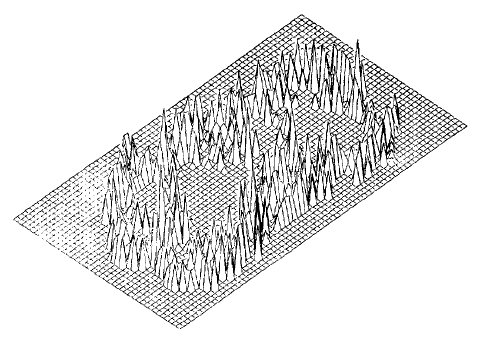
\includegraphics[width=\linewidth]{Figures/Occupancy_Grid_Map/Occupied_Areas_in_Map}
		\caption{This figure shows the occupied areas in the map where the height of the peaks shows the occupancy certainty factors.\cite{moravec1985high}}
		\label{fig:OGMwothresh}
	\end{subfigure} \hspace{0.1\textwidth}
	\begin{subfigure}[t]{0.4\linewidth}
		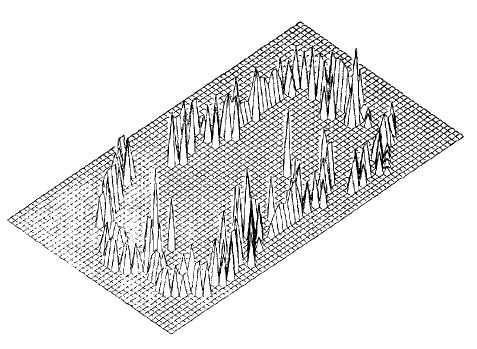
\includegraphics[width=\linewidth]{Figures/Occupancy_Grid_Map/Occupied_Areas_in_Map_after_Thresholding}
		\caption{This figure shows the occupied areas in the map after thresholding the occupancy certainty factors.\cite{moravec1985high}}
		\label{fig:OGMwthresh}
	\end{subfigure}
	\caption{Thresholding of the occupancy grid map data.}
	\label{fig:OGMw-wothresh}
\end{figure}


\subsubsection{Bayesian update with forward sensor model}
The forward sensor model is formulated in formula \ref{eqn:for_sens}. When comparing to the inverse sensor model, this model also makes the static world assumption (i.e. a measurement is conditionally independent from the previous measurements and poses), but does not assume that the grid cell's are conditionally independent. It is a generative model that is modeled as a likelihood. Given the world that is represented by the \gls{OGM} $m$, and the complete set of poses $x_{1:T}$, this formula would give the most likely set of sensor measurements $z_{1:T}$ \cite{carvalho2013comparative}.

\begin{equation} \label{eqn:for_sens}
	p(z_{1:T}|m,x_{1:T})
\end{equation}

To find the \gls{OGM}, the likelihood formula \ref{eqn:for_sens} needs to be maximized by iteratively adjusting $m$. To do so, a reliable sensor model needs to be made.
Not all measurements are caused by obstacles, some are erroneously made. Therefore, it is assumed that all sensor measurements, $z$, can be subdivided into the following three cases to model the sensor. \cite{thrun2003learning} \cite{carvalho2013comparative}.  

\begin{enumerate}
	\item \textbf{Non-random:} A non-random measurement is caused by an obstacle that lies within the sensor's range.
	\item \textbf{Random:} A random measurement covers the remaining causes of a sensor measurement such as specular reflections or false positives.
	\item \textbf{Maximum reading:} When the sensor does not detect an obstacle it will return a value that is equal to the maximum range $z_{max}$ of the sensor.
\end{enumerate}

These cases can be modeled using binary correspondence variables, $c_{t,k}, c_{t,*}$ and $c_{t,0}$ respectively, which are linked to their specific probability values. The respective correspondence variable is equal to $1$ if the measurement corresponds to that particular case. This in turn determines the conditional probability of the measurement given the $c_t$ value, which results in equation \ref{eqn:condition_ct} \cite{thrun2003learning} \cite{carvalho2013comparative}

\begin{equation} \label{eqn:condition_ct}
	p(z_t, c_t|m,x_t) = p(z_t|m,x_t,c_t)p(c_t|m,x_t)
\end{equation} 

where 
\hfill \break
\begin{equation} \label{eqn:correspondence_var}
	p\left(c_{t} \mid m, x_{t}\right)=\left\{\begin{array}{ll}
		p_{\text {rand }} & \text { if } c_{t, *}=1 \\
		p_{\max } & \text { if } c_{t, 0}=1, K_{t} \geq 1 \\
		\left(1-p_{\text {rand }}-p_{\max }\right) \prod_{i=1}^{k-1}\left[\left(1-p_{h i t}^{(i)}\right)\right] p_{h i t}^{(k)} & \text { if } c_{t, k}=1, k \geq 1
	\end{array}\right.
\end{equation}
\hfill \break

and where $p_{rand}$ is the random probability, $p_{max}$ is the maximum reading probability, and $p_{hit}$ is the probability function of the obstacle's coverage within the sensor. $K_t$ and $k$ are the total number of obstacles and an obstacle instance respectively. By taking the logarithm of equation \ref{eqn:condition_ct} and regarding the complete set of sensor data, the expected log-likelihood can be computed. The \gls{OGM} $m$ can be found when the log-likelihood is maximized using the Expectation Maximization(EM) algorithm. However, this algorithm requires a high computational effort, which makes it impossible to perform real-time on \glspl{AV} compared to the inverses sensor model \cite{thrun2003learning}. Recent research uses maximum a posteriori (MAP) inference instead of the EM algorithm to increase the convergence speed of the \glspl{OGM}, but real-time performance has not yet been acquired \cite{dhiman2014modern}.


\subsubsection{Comparison of the sensor models} \label{subsub:comp_sens_mod}
In this subsection, the inverse and forward sensor models are compared. Figure \ref{fig:OGM_inv_for_comp} shows the difference between the inverse sensor model and the forward sensor model, which can be compared to the ground truth. 

\begin{figure}[h!]
	\centering
	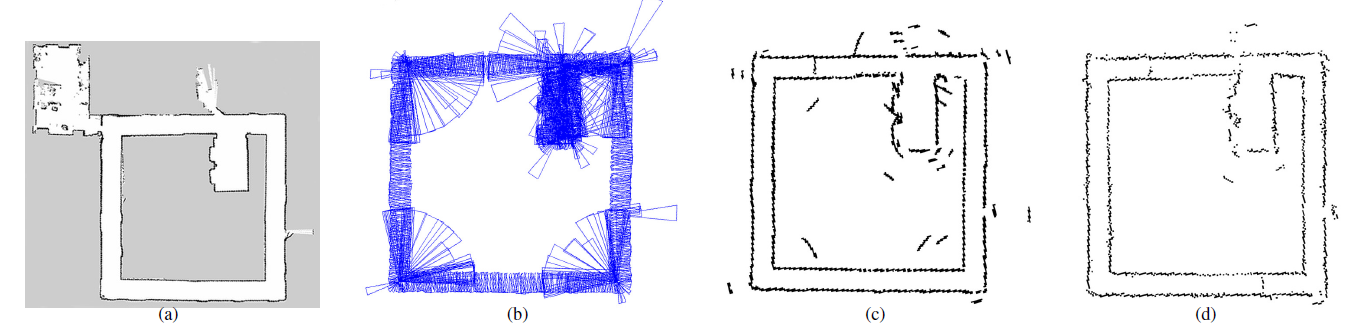
\includegraphics[width=1\linewidth]{Figures/Occupancy_Grid_Map/OGM_inverse_forward_compare}
	\caption{The experimental results from Carvalho's research \cite{carvalho2013comparative} which compares the inverse sensor model with the forward model. Figure (a) is the ground truth map. Figure (b) are the taken measurements. Figure (c) is the computed \gls{OGM} using the inverse sensor model. Figure (d) is the computed \gls{OGM} using the forward sensor model.}
	\label{fig:OGM_inv_for_comp}
\end{figure}

The forward sensor model is more accurate but also requires much more computational effort \cite{carvalho2013comparative}. Both probabilistic methods have in common that they cannot tell the difference between incompleteness (i.e. ignorance) and uncertainty. When the occurrence of an event does not hold absolute confidence, this lack of confidence can have two causes. The first cause could be that due to a lack of information another possible event is not excluded. This lack of information is defined as ignorance. A second cause could be that the occurrence of the event is not definitely true, which is defined as uncertainty \cite{liu2001propositional}.
The \glsfirst{DST} \cite{dempster1967upper} \cite{shafer1976mathematical}, however, can distinguish between ignorance and uncertainty. This theory can be used to generate better \glspl{OGM}. In the following subsection, evidential occupancy grid mapping, using the \gls{DST}, will be explained.


\subsection{Evidential Occupancy Grid Mapping} \label{subsec:evid_OGM}
In evidential Occupancy Grid Mapping, the \glsfirst{DST} is used to estimate the state of the occupancy grid cells. This method, as opposed to the probabilistic method, can distinguish ignorance (the cell is either empty or occupied) from uncertainty (there is evidence that the cell is both empty and occupied with a certain belief). However, more computational power is required to for the evidential method compared to the probabilistic method \cite{moras2014evidential}. The following section will first explain the mathematics behind \gls{DST}. Then, its application on \glspl{OGM} is discussed. 


\subsubsection{The Dempster-Shafer Theory}
The DST formalizes the transferable belief model. The model defines a discrete \gls{FOD} which contains the set of possible states of a system. In the case of an \gls{OGM}, the \gls{FOD} is $\Omega = \{E, O\}$, with $E$ for Empty and $O$ for Occupied. A mass function $M$ is defined that maps the powerset $2^\Omega$ of $\Omega$ to the domain $[0 \; 1]$. The powerset is the set of all subsets of $\Omega$ including the empty set $\emptyset$ and itself ($2^\Omega = \{\emptyset, E, O, \Omega \}$). If $A$ is an element in $2^\Omega$, then $M(A)$ represents the amount of evidence (mass) that supports hypothesis $A$ within the domain $[0 \; 1]$. Then, two properties are set to the mass function $M$. First, $M(\emptyset) = 0$, and second, formula \ref{eqn:sum_massfunc} verifies that the sum of the masses of each hypothesis in the powerset is equal to $1$. This means that it is assumed that the powerset $2^\Omega$ is complete and that no evidence will be obtained that supports none of the hypotheses in the \gls{FOD}. A mass function with these two properties is called a \gls{BBA} mass function. \cite{moras2014evidential}. A \gls{BBA} mass function allows for the assignment of lower and upper bounds of a probability interval, belief $Bel()$ and plausibility $Pl()$ respectively, that represent the support to the hypotheses $A \in 2^\Omega$.

Belief is the sum of the masses of all the hypothesis's subsets including the hypothesis, as is shown in equation \ref{eqn:belief_func}, where $A$ and $B$ represent hypotheses (e.g. for the $\Omega$-hypothesis, this would be the mass of $\Omega$ and the subsets of $\Omega$: $E$ and $O$]).
In equation \ref{eqn:plaus_func} it can be seen that the plausibility is computed by taking $1$ minus the sum of the masses that exclude the hypothesis (e.g. for the hypothesis $O$, the plausibility $Pl(O)$ would be $1$ minus $M(\emptyset)$ and $M(E)$ which is $0.3$). \cite{moras2014evidential}.

\begin{equation} \label{eqn:sum_massfunc}
	\sum_{A \in 2^\Omega}^{} M(A) = 1 
\end{equation}

\begin{equation} \label{eqn:belief_func}
	Bel(A) = \sum_{B|B \subset A}^{} M(B) 
\end{equation}

\begin{equation} \label{eqn:plaus_func}
	Pl(A) = \sum_{B|B \cap A \not = \emptyset}^{} M(B) = 1 - \sum_{B|B \cap A = \emptyset}^{} M(B) 
\end{equation}

\hfill \break

An example of a \gls{BBA} mass function is shown in table \ref{tab:belief_func_example}, given the powerset $2^\Omega = \{\emptyset, E, O, \Omega \}$. In this example, a sensor reading obtains information that a certain grid cell is empty. The sensor reading's probability of being reliable is $0.7$ and $0.3$ for being unreliable. This information can be used to assign a subjective probability (mass) to each hypothesis, which sum up to $1$. A reliable sensor will give a true reading, so the hypothesis of the grid cell being empty ($m(E)$) is assigned a mass of $0.7$. However, given that there \textit{is} a grid cell ($m(\emptyset) = 0$), the sensor reading has a probability of $0.3$ that it is unreliable. This does not mean that the grid cell is occupied with a probability of $0.3$, but it means that it's state is uncertain with that probability. Therefore, a mass of $0.3$ is assigned to the hypothesis $m(\Omega)$ that states that the grid cell is either empty or occupied. The hypothesis of the cell being occupied ($m(O)$) will have a mass of $0$, since there is no evidence that supports it. \cite{shafer1992dempster}. Subsequently, the belief $Bel()$ and the plausibility $Pl()$ of the hypotheses are computed, giving the lower and upper probability bounds for the hypotheses. 


\begin{table}[h!]
	\begin{center}
		\caption{An example of a \gls{BBA} mass function.}
		\begin{tabular}{llll} 
			\toprule[0.25ex]
			Hypothesis & Mass & Belief & Plausibility \\ [0.5ex]
			\midrule 
			$M(\emptyset)$ & 0 & 0 & 0 \\ 
			$M(E)$ & 0.7 & 0.7 & 1.0 \\
			$M(O)$ & 0 & 0 & 0.3 \\
			$M(\Omega)$ & 0.3 & 1.0 & 1.0 \\
			\bottomrule[0.25ex]
		\end{tabular}	
		\label{tab:belief_func_example}
	\end{center}
\end{table}

\subsubsection{Applying \gls{DST} to generate \glspl{OGM}}
To generate an evidential \gls{OGM}, given independent sensor data, each grid cell is assigned a mass function $M_{i,j}$ with beliefs and plausibilities. If new sensor data about a grid cell is obtained, the DST method can fuse the mass functions of the current cell state and the new sensor data according to the joint mass equations \ref{eqn:fuse_dst} and \ref{eqn:conj_rule}. \cite{moras2014evidential}.

\begin{equation} \label{eqn:fuse_dst}
	M_1 \oplus M_2 (A) = \left \{ 
	\begin{array}{ll} 
	\frac{M_{1 \cap 2}(A)}{1 - M_{1 \cap 2}(\emptyset)} & A \not = \emptyset \\
	0	&	 A = \emptyset
	\end{array} \right \}
\end{equation}

Where $\cap$ is the conjunctive rule with $B$ and $C$ hypotheses and $A$ the joint hypothesis:

\begin{equation} \label{eqn:conj_rule}
	M_{1 \cap 2}(A) = \sum_{B, C \in 2^\Omega | A = B \cap C}^{} M_1(B) \cdot M_2(C)
\end{equation}

Then, a probability measure can be taken from the mass function according to equation \ref{eqn:belief_2_prob}. Here, $A$ and $B$ represent hypothesis subsets of powerset $2^\Omega$. The cardinality (number of elements in a subset) is denoted as two vertical bars $\vert \vert$.

\begin{equation} \label{eqn:belief_2_prob}
	P(A) = \sum_{B \in 2^\Omega}^{} M(B) \cdot \frac{\vert A \cap B \vert}{\vert B \vert}
\end{equation}

This equation is not bijective, meaning an infinite number of mass functions can be found given the same probability. This is because information that distinguishes ignorance from uncertainty is lost when the mass function is transformed to a probability. This lost information in probabilities is exactly what makes the DST method a more accurate but also a more computational method for \gls{OGM} generation. \cite{moras2014evidential}. The processing time of the DST method is about $1.5$ times higher than that of the inverse sensor model probabilistic method \cite{ribo2001comparison}. Figure \ref{fig:OGM_prob_DST_comp} shows the qualitative differences between the probabilistic approach (center) and the DST approach (right).  

\begin{figure}[h]
	\centering
	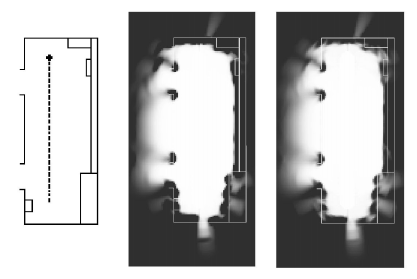
\includegraphics[width=0.6\linewidth]{Figures/Occupancy_Grid_Map/OGM_prob_l_DST_r_compare}
	\caption{Ribo and Pinz \cite{ribo2001comparison} compare the probabilistic method (center) with the DST method (right) to generate OGMs. The ground truth schematic is shown left.}
	\label{fig:OGM_prob_DST_comp}
\end{figure}

\newpage

\subsection{Alternative methods for Occupancy Grid Mapping} \label{subsec:alt_OGM}
Besides the probabilistic and evidential approach to generate \glspl{OGM}, there are more methods to determine which cells in the grid are occupied. Two methods, the possibilistic method and the \gls{NN} method are discussed in this section. These methods are less common than the probabilistic and evidential methods, therefore they are not explained in depth in this literature review. For more in depth information about the methods it is advised to read the papers from which the methods are cited. At the end of this section comparison methods of OGMs are discussed. 

\subsubsection{Possibilistic Occupancy Grid Mapping}
Oriolo \cite{oriolo1997fuzzy} defines the \gls{OGM} as two fuzzy sets where one set is empty ($E$) and the other occupied ($O$). Based on measurements, each cell is assigned a partial membership to states $E$ and $O$. This partial membership allows to process and distinguish insufficient (ignorance) from uncertain information. Ribo and Pinz \cite{ribo2001comparison} compare this fuzzy method (also called possibilistic) with the probabilistic and evidential methods and conclude that the possibilistic method is more conservative and thus more robust towards outliers compared to the other two methods. However, its robustness also causes loss of information and the emergence of artifacts. Like the DST method, the possibilistic method requires about $1.5$ times more computation time than the inverse sensor model probabilistic method. 

\subsubsection{\gls{NN}-based Occupancy Grid Mapping}
Thrun \cite{thrun1993exploration} uses an \glsfirst{NN} to generate an \gls{OGM} from measurements. In a simulated environment, the \gls{NN} is trained to interpret sensor data and estimate a confidence that a cell is occupied. This trained \gls{NN} is then tested in a real environment and shows it can model unknown environments efficiently, however the network cannot be trained until convergence because then it would overfit on the simulated environment and perform worse in real situations. Collins \cite{collins2007occupancy} compares the \gls{NN} method with the probabilistic method. The \gls{NN} method performs worse that the probabilistic one because it has a tendency to overestimate the free space beyond the actual environment borders. It also tends to model the sensor's extremities (maximum value due to no detection) as occupied areas, while the probabilistic approach's algorithm will ignore these extremities. Van Kempen \cite{van2021simulation} takes the use of \glspl{NN} to generate OGMs even further. Van Kempen proposes a deep inverse sensor model together with a PointPillars architecture (often used to process LiDAR data) extended with an evidential prediction head to estimate an evidential \gls{OGM}, including the uncertainties. The network is trained using a synthetic dataset. The network is then tested on synthetic data and on real-world data. It shows promising results on both synthetic data and real-world data. It performs better than classical approaches on the synthetic data, but the generalization capabilities are not sufficient yet to have accurate results on the real-world data. In future research, van Kempen suggests to use a more diverse dataset to train the network on for better generalization. 

\subsubsection{Comparison methods for \glspl{OGM}}
Metrics to measure and decide what \gls{OGM} generation method is the best are not easy to define. The computation time and memory requirements to generate the \gls{OGM} can be determined and used as a metric to compare efficiency of the \gls{OGM} methods. Most other methods to determine and compare the quality of \glspl{OGM} are qualitative (visual inspection) \cite{ribo2001comparison}. Collins \cite{collins2007occupancy} summarizes some quantitative metrics based on image similarity measures and one that bases the \gls{OGM} quality on the usefulness of the map for a robot to find paths, compared to the ground truth. More about metrics to evaluate \glspl{OGM} will be discussed in section \ref{sec:metrics}. \\

Besides ways to generate the traditional \gls{OGM} maps that provide information about the cell occupancy, there are extended \gls{OGM} forms that contain more information. The next subsections will elaborate on some of those extended forms.


\subsection{Occupancy Grid Map extended forms} \label{subsec:OGM_ext_form}
Many variations of the \gls{OGM} have been invented and researched that represent environments in more complex methods, including for example 3D information \cite{degerman20163d}, semantic segmentation of the cells \cite{lu2019monocular}, or dynamic information of the occupied regions \cite{nuss2018random}. 

\subsubsection{3D Occupancy Grid Mapping}
Degerman \cite{degerman20163d} proposes a way to create 3D Occupancy Grid Maps using 3D RADAR data. Degerman uses a binary Bayes filter to estimate the occupancy probabilities of the assumed independent voxels (grid cells in 3D). The RADAR data is obtained in spherical coordinates (radius $r$, scanning angle $\theta$, and azimuth angle $\phi$) after which those measurements are mapped to the Cartesian coordinates of the 3D \gls{OGM}. As shown in Figure \ref{fig:OGM3Dspherical}, the spherical measurement grid cells are dense in short range while the distances between them increase for longer ranges. Therefore trilinear interpolation is used to combine the spherical data points when they are mapped to the Cartesian coordinates. An example of the resulting 3D occupancy grid is shown in Figure \ref{fig:OGM3Dex}.


\begin{figure}[h]
	\centering
	\begin{subfigure}[t]{0.4\linewidth}
		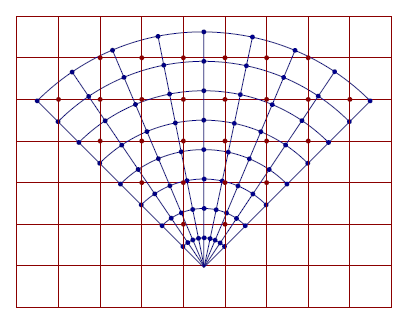
\includegraphics[width=1\linewidth]{Figures/Occupancy_Grid_Map/3D_Occupancy_Grid_Spherical_Coord}
		\caption{The 2D image of the measured spherical grid points (blue) and the Cartesian grid points that are computed by performing interpolation on the surrounding spherical points. \cite{degerman20163d}}
		\label{fig:OGM3Dspherical}
	\end{subfigure} \hspace{0.1\textwidth}
	\begin{subfigure}[t]{0.4\linewidth}
		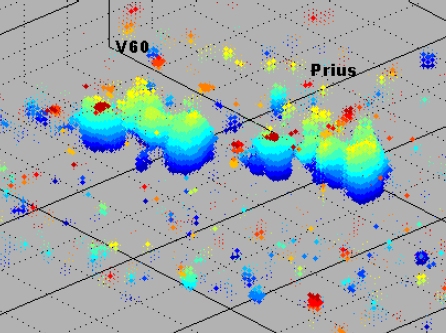
\includegraphics[width=1\linewidth]{Figures/Occupancy_Grid_Map/3D_Occupancy_Grid_example}
		\caption{An example of a 3D occupancy grid where each voxel with a likelihood value above a certain threshold is visualized. The blue color represents lower levels while the red color represents higher levels. The clusters of occupied voxels represent two cars (V60 and Prius). \cite{degerman20163d}}
		\label{fig:OGM3Dex}
	\end{subfigure}
	\label{fig:OGM3Dboth}
\end{figure}




\subsubsection{Semantic Occupancy Grid Mapping}
While classical OGMs only contain information about occupancy, Lu \cite{lu2019monocular} proposes a method that utilizes the semantics of the environment in an \gls{OGM}. The method they propose is an end-to-end convolutional neural network with a variational autoencoder-decoder part that takes monocular RGB camera data as input and outputs an \gls{OGM} with an additional semantics channel. They distinguish the environment with four labels: road, sidewalk, terrain, non-free space. The network is trained and evaluated on the Cityscapes \cite{cordts2016cityscapes} and KITTI \cite{geiger2013vision} datasets and the results show that the network is robust to sparse input data and a weak ground-truth. Figure \ref{fig:sem_OGM} shows an illustration of the semantic \gls{OGM} method.

\begin{figure}[h]
	\centering
	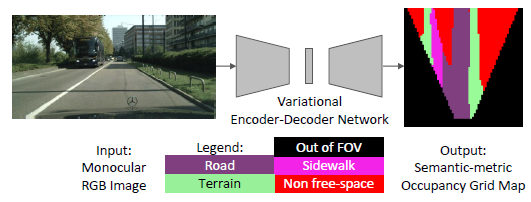
\includegraphics[width=0.7\linewidth]{Figures/Occupancy_Grid_Map/Semantic_OGM_Network}
	\caption{An illustration of the semantic \gls{OGM} method that takes a monocular RGB image as input and outputs a semantic \gls{OGM} \cite{lu2019monocular}.}
	\label{fig:sem_OGM}
\end{figure}


\subsubsection{Dynamic Occupancy Grid Mapping}
Besides having information about semantics in an \gls{OGM}, for purposes such as motion planning and tracking, information about the environment's dynamics is also desired. 
Danescu \cite{danescu2011modeling} proposes a particle based method for tracking the dynamic driving environment in occupancy grids. This method represents the world as a 2D BEV grid in which each obstacle is represented by a set of particles that are located in the grid's cells. Each particle has their own position and speed and can move between cells based on their dynamics. Also, particles can be created or destroyed over time. The occupancy probability of a cell $C$ is estimated by the ratio of the number of particles in that cell and the total number of particles allowed for a single cell $N_C$.
The number of particles allowed for a single cell is predetermined, while the total number of particles in the grid, $N_S$ is not fixed and is dependent on the number of obstacles in the environment.
By taking the average speed of all particles within a grid cell, the speed estimation of that cell is estimated. If obstacles in the environment overlap, the particles in a single cell can have different speeds. Clustering of the speeds can be used to model the speeds of multiple obstacles that overlap in a cell. This way, a tracking algorithm is used to create, update, and destroy particles to estimate the occupancy and dynamic state of the real world. These states generally are saved in separate channels of the grid, one for the occupacy state, and two for the speed and orientation of the grid cells. \\

Nuss \cite{nuss2018random} continues this research and proposes an improved method, using the Dempster-Shafer theory, to assign particles to grid cells. They name this method the Dynamic Occupancy Grid Map (DOGMa). An example is shown in figure \ref{fig:DOGMa_example}.

\begin{figure}[h]
	\centering
	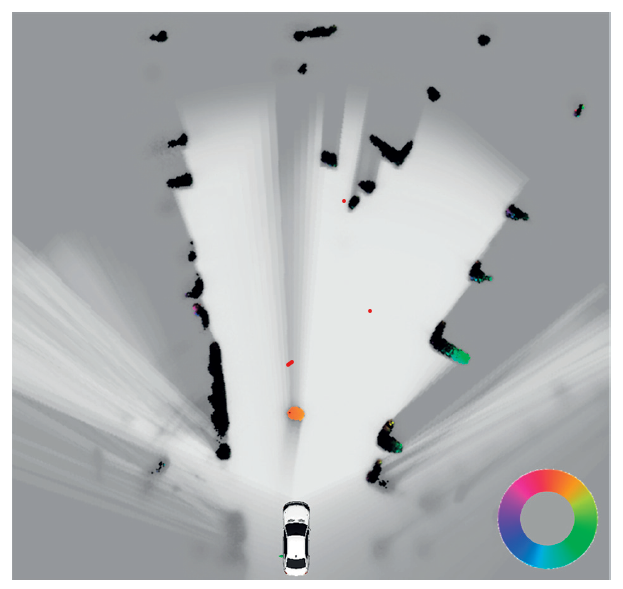
\includegraphics[width=0.4\linewidth]{Figures/Occupancy_Grid_Map/DOGMa_example}
	\caption{A Dynamic Occupancy Grid Map example in which the static parts (occupancy information) are shown in black and white, with black occupied and white emtpy space. The dynamic information is shown in color. The color code represents the direction of the grid cell corresponding to the color wheel at the bottom right. The saturation value of the color determines the velocity, where the velocity is higher if the saturation is higher. \cite{nuss2018random}.}
	\label{fig:DOGMa_example}
\end{figure}

Besides the 3D \gls{OGM}, semantic \gls{OGM} and the DOGMa, there are more variations to occupancy grid maps. In some papers, the term \gls{OGM} is not used however, making it sometimes hard to define what is still an \gls{OGM} and what isn't. 
For example, Wu \cite{wu2020motionnet} proposes a method to predict future environments using Bird's Eye View (BEV) maps. The paper states that they define an alternative to OGMs, which they call a BEV map. The BEV map is a grid map with discrete occupancy information in each cell. The BEV map has multiple channels. Each channel represents another height layer of the environment, which basically means that the whole BEV map is a 2D pseudo-image, because all layers together form a 3D representation of the environment. In principle, this approach is similar to a 3D \gls{OGM}. In Wu's method, a Deep Learning Network is used to apply semantics to the BEV map and estimate temporal features (the dynamics). In essence, Wu's method creates OGMs that are 3D and incorporate semantics and dynamics. In this literature review, environment representations such as Wu's are also considered \gls{OGM} variations. \\

\subsection{What OGM form is most suitable to use in OGM prediction methods?} \label{subsec:OGM_conclude}

What \gls{OGM} form is best depends on the requirements of the prediction method. Table \ref{tab:ogm_overview} shows an overview of the different \gls{OGM} generation methods. In the case of \glspl{AV}, there will be a trade-off between accuracy and computation time. If a fast method is desired, the inverse probabilistic method would be the best choice. The downside is that the accuracy will be lower compared to most other methods and there is no distinction between ignorance and uncertainty. If a higher accuracy is desired and there is the means to carry a higher computational load, the \gls{DST} or possibilistic generation methods are more suitable because of their high accuracy and distinction of ignorance and uncertainty. The possibilistic method is more conservative than the \gls{DST} method, which results in fewer outliers but more artifacts and information loss in the \glspl{OGM} compared to the \gls{DST} method. In the context of \glspl{AV}, having artifacts in the \glspl{OGM} and a higher information loss both might result in dangerous situations in which the \gls{AV} either perceives something that is not present, or does not perceive something that is present. Therefore, the best option would be the \gls{DST} method. Due to the high computational effort of the forward sensor model, and because the \gls{NN}-based method is not developed enough to acquire a good accuracy in real situations, these options are considered the least suitable for \gls{OGM} prediction purposes. 	 


\begin{table}[h!] 
	\caption{This table gives an overview of the properties of each \gls{OGM} generation method based on the information in this chapter.}
	\centering
	\resizebox{\linewidth}{!}{%
		\begin{tabular}{llll} 
			\toprule[0.25ex]
			& \textbf{Accuracy} & \textbf{Computation Effort} & \textbf{Ignorance-Uncertainty Distinction} \\ 
			\midrule
			\textbf{Inverse Probabilistic} & Average & Low & No \\
			\textbf{Forward Probabilistic} & High & High & No \\
			\textbf{\gls{DST}} & High & Average & Yes \\
			\textbf{Possibilistic} & High & Average & Yes \\
			\textbf{Neural Network Based} & Low & Unknown & Yes \\
			\bottomrule[0.25ex]
		\end{tabular}
	}
\label{tab:ogm_overview}
\end{table}

Further, regarding the extended forms, each extension will provide the \gls{OGM} with more information. Generally, when performing predictions, having more information will result in better predictions. The trade-off in this case is again one of accuracy versus computation effort. Whether the amount of additional information is worth the additional computation effort depends on the goal of the predictions. \\

The next section will discuss the available datasets that are used to obtain Occupancy Grid Maps from for research and what metrics are used to determine the accuracy of those OGMs. 


	\newpage
	\section{Datasets} \label{sec:datasets}
When using deep learning networks, it is important to choose a dataset (or multiple datasets) that optimally fulfills the requirements for its purpose. The dataset will be used to train and evaluate the deep learning network on. So, if the dataset is faulty, the resulting model will be faulty as well. A faulty model will predict faulty \glspl{OGM}, which could cause dangerous situations if it is used by an \gls{AV} and affects its decisions regarding motion planning. This chapter first discusses what the requirements are for a dataset that is used for \gls{OGM} prediction. Then, based on those requirements, nine criteria are devised that are used to evaluate the adequacy of a dataset. Subsequently, ten datasets are evaluated against the criteria and compared with one another. A dataset top 3 is presented in this chapter's conclusion in which the question \airquote{\textit{What dataset is most suitable to generate \gls{OGM} sequences for \gls{OGM} prediction?}} is answered. \\

In the case of \gls{OGM} prediction in a traffic scene context, literature provides (almost) no criteria which a dataset for this purpose should meet. Therefore, this literature study provides its own criteria for a \gls{OGM} prediction dataset, based on practical reasons and broader literature about datasets. \\

A dataset is desired that contains \gls{BEV} environmental data of ego-vehicle centered traffic scenes that can be used to generate \gls{OGM} sequences. Moreover, if the dataset contains data that can be used to generate an extended form of the \gls{OGM}, as is discussed in chapter \ref{sec:ogm}, it would be beneficial.
It is important that the dataset's traffic scenes reflect the diversity of real world situations. The way a dataset's data is sampled from a population can influence how much the dataset reflects reality. A model that is trained on biased data could generate inaccurate predictions \cite{mehrabi2019survey}. If a traffic scene dataset is obtained in only one geographic, environmental, or cultural location, the dataset will contain some kind of bias towards the behavior, representation, and environmental context of that location \cite{mehrabi2019survey}. For example, \cite{nordfjaern2010investigation}'s research shows that geographical location (rural vs urban), and factors such as age, gender, and education influence the behavior of drivers. Also, \cite{nordfjaern2014culture} shows that traffic risk perception differs per culture and country. This can result in different traffic behavior between countries given the same traffic scene context. It is therefore important that a dataset contains data from multiple locations in varying geographical, cultural, and environmental areas. Also, the dataset should be diverse in the kind of traffic participants it contains. Besides vehicles and pedestrians, it is desired that the dataset contains other traffic participant classes (e.g. cyclists, riders). The more diverse the dataset is, the smaller the dataset bias is, and the better the prediction accuracy is of the model that is trained on that dataset. Besides having diverse data, the performance of a deep learning network also increases with a logarithmically increasing dataset size \cite{torralba2011unbiased}. Therefore, a dataset should be large besides being diverse. For large-scale datasets, even rare traffic cases are expected to be captured enough times so the deep learning network can generalize those situations accurately. \\

Regarding the traffic scene sequences, literature does not mention the ideal frame rate that \gls{OGM} sequences should have to generate optimal predictions, \cite{chen2007review} reviewed literature on what the influence of frame rate of visual perceptions is on human perceptual performance. In \cite{chen2007review}'s reviewed papers, humans are situated in virtual environments in which the visual information of the environment is updated at a variable frame rate. The research shows that higher frame rates increase the performance (accuracy, reaction time, recognition) at which humans completed certain perceptual tasks. Frame rates below 10 Hz showed sharp performance degradations, while frame rates higher than 15 Hz did not increase performance significantly. Therefore, a frame rate of 10 Hz is considered the minimum threshold for accurate human perceptual understanding. Using humans as reference for the performance of deep learning networks, a frame rate of 10 Hz is also considered as the minimal threshold for accurate \gls{OGM} prediction. So, it is desired that a dataset has at least a 10 Hz sampling rate of its environment. Furthermore, the traffic scene sequences should be long enough. The sequences have to be split into a part that represents the 'past' to use as input sequences for the deep learning network, and a ground truth of the 'future' to compare the predictions with. The research by \cite{lange2020attention} uses $0.5$s of past \glspl{OGM} to predict up to $1.5$s of future \glspl{OGM}. So, a sequence of $2$s is sufficient to perform \gls{OGM} prediction using this method. If a margin of $0.5$s is considered for the length of the past information and for the length of the prediction horizon, a dataset should provide \gls{OGM} sequences of at least $3$s long. \\

Aside from the contents of the dataset, the quality of the sensors with which the dataset is recorded is essential. The resolutions of the sensors should be high enough to capture the smallest traffic participant's (\glspl{VRU}) behavioral patterns. Not only the performance of deep learning network, but also the time that is required to pre-process, train, and evaluate the network is greatly dependent on what dataset is used. Also, the performance of a network should be compared reliably. Therefore, it is important that a dataset is chosen which other research has based their network training and evaluation on, so there are enough results for reliable comparisons. \\

To ensure that the optimal dataset is chosen for \gls{OGM} prediction research, the following list of criteria is devised which a dataset has to meet in order to be suitable for \gls{OGM} prediction. Based on how the dataset scores on this list, an informed decision can be made. 

\begin{enumerate}
	\item The dataset contains data of ego-vehicle centered traffic scene sequences that provide at least 2D \gls{BEV} information of the environment.
	\item The dataset provides enough diverse data to train and evaluate a network on.
	\item The dataset contains traffic scene sequences, or provides means to easily generate them.
	\item The sequences have enough frames per sequence and a frame rate that is suitable for capturing road user behavior and trajectories.
	\item The sequences contain various traffic actors including vehicles and \glspl{VRU}.
	\item The dataset data, and any \gls{OGM} that can be generated from it, provides a resolution that is high enough to distinguish and to track \glspl{VRU}. 	
	\item The sequences show a diversity in environmental properties, containing \glspl{VRU}, that may influence the generated \glspl{OGM} (e.g. urban vs rural, dense vs sparse traffic).
	\item The dataset provides data, including ground truth, that is required for generating extended \gls{OGM} forms.
	\item Results of other research using the dataset for generating and predicting \glspl{OGM} is available for comparison. 
\end{enumerate}


A total of ten datasets coming from three categories are found that contain ego-vehicle centered traffic scene sequences. Three datasets were created for a purpose that includes motion prediction. Five datasets were created for object detection purposes. The last two datasets were mainly created to research semantic segmentation on. All the datasets are recorded using a vehicle equipped with one or multiple sensors that drives through real traffic. \\

To evaluate the datasets against the criteria, information about each dataset is gathered and put into a table (see table \ref{tab:datasets_overview}). The first criterion is met if the dataset contains 2D \gls{BEV} information about the environment. From the recording vehicle's point of view, having 2D \gls{BEV} information means that the vehicle should gather 3D sensor data which can be projected onto the 2D top view plane. The information about the sensors provides the data to evaluate this first criterion. The second criterion is tested using information about the number of categories and classes that are labelled in the datasets. If the dataset contains sequences of its sensor data, the third criterion is met. The fourth criterion is tested by evaluating the sampling frequency and length of the sequences. To test the fifth criterion, the number (and presence) of vehicles and pedestrians is evaluated. The information about the sensors is used to test the sixth criterion. The seventh criterion is evaluated by examining the diversity of sampling locations. Then, the eighth criterion is met if the dataset contains data to generate extended \glspl{OGM}. Finally, the ninth criterion is tested by evaluating whether there exists literature that generates \glspl{OGM} from the dataset and whether there is literature that uses those generated \glspl{OGM} for \gls{OGM} prediction. The evaluation and comparison of each dataset against the criteria is shown in table \ref{tab:datasets_criteria}. \\

The most interesting characteristics of each dataset are highlighted below in three subsections based on the dataset's original purposes: Motion prediction (section \ref{subsec:data_track_mot}), Object Detection (section \ref{subsec:data_ob_det}), and Semantic Segmentation (section \ref{subsec:data_sem_seg}). At the end of this chapter (section \ref{subsec:data_con}) a conclusion about the datasets is provided.


\subsection{Tracking and Motion prediction Datasets} \label{subsec:data_track_mot}
The following three datasets are obtained for tracking or motion prediction purposes. The \gls{STIP} dataset \cite{liu2020spatiotemporal}, the Argoverse dataset \cite{chang2019argoverse} and the RobotCar dataset \cite{robotcardatasetijrr}. \\

The \gls{STIP} dataset \cite{liu2020spatiotemporal} is obtained using three cameras (left, front and right) with a 1216x1936 resolution at 20 Hz positioned on the recording vehicle. An example of the \gls{STIP} dataset's camera images is shown in figure \ref{fig:dat_stip}. However, these are not stereo cameras, so no 3D information is obtained. This dataset does therefore not meet the first criterion. 3D information can be computed from the monocular images using monocular unsupervised depth estimation techniques \cite{godard2017unsupervised}. However, this probably will not yield as reliable results compared to stereo vision data and the time spent on generating 3D data could also be spent on training a network using a dataset that does contain 2D \gls{BEV} information. A remarkable property of this dataset is that the sampling frequency of the camera images is 20 Hz. When comparing the \gls{STIP} dataset's sampling rate to the other dataset's rates (see table \ref{tab:datasets_overview}, it can be seen that this dataset, together with the \gls{ECP2.5D} \cite{braun2020ecp2} dataset has the highest sampling rate. \\

\begin{figure}[h!]
	\centering
	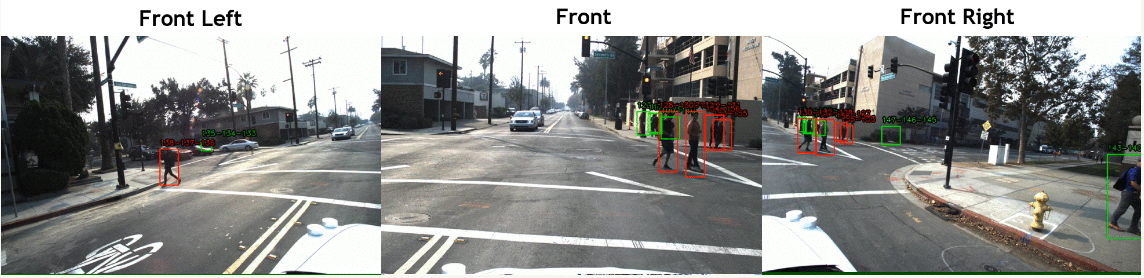
\includegraphics[width=0.8\linewidth]{Figures/Datasets/STIP_Dataset}
	\caption{This image shows an overview of the \gls{STIP} \cite{liu2020spatiotemporal} dataset's camera images. Pedestrians are annotated with cross (red) not-cross (green) labels.  \cite{liu2020spatiotemporal}}  
	\label{fig:dat_stip}
\end{figure}

The Argoverse dataset \cite{chang2019argoverse} is recorded in only two cities in one country. It therefore contains little geographic diversity compared to the \gls{ECP2.5D} \cite{braun2020ecp2} and Cityscapes \cite{cordts2016cityscapes} datasets. On the other side, the Argoverse dataset \cite{chang2019argoverse} contains 333K 5-second sequences and labels 17 different classes, including vehicles, pedestrians and cyclists. Furthermore, \cite{roddick2020predicting} has already used this dataset to generate \glspl{OGM}. Examining \cite{roddick2020predicting}'s research could therefore speed up the \gls{OGM} generation time. \\

The RobotCar dataset \cite{robotcardatasetijrr} is collected in only one city and no data is labeled. It is therefore not a diverse dataset compared to the other datasets. The dataset contains 360-second sequences, but of an unkown number. What is beneficial about this dataset is that \cite{dequaire2018deep} and \cite{wang2020l2r} used it for \gls{OGM} generation before, where \cite{dequaire2018deep} also performed \gls{OGM} prediction.


\subsection{Object Detection Datasets} \label{subsec:data_ob_det}
This subsection will discuss five datasets that were originally obtained for object detection purposes. The \gls{ECP2.5D} dataset \cite{braun2020ecp2}, the \gls{BDD100K} dataset \cite{yu2020bdd100k}, the \gls{KITTI} dataset \cite{geiger2012we}, the nuScenes dataset \cite{caesar2020nuscenes}, and the Waymo Open dataset \cite{sun2020scalability}. \\

The \gls{ECP2.5D} dataset \cite{braun2020ecp2} contains 15-second sequences in which seven different classes are labeled. This is average compared to the other datasets. This dataset is remarkable because it is recorded in 31 cities in 12 countries which makes this the most diverse datatset regarding geographic locations. Also, the sampling frequency of the sequences is 20 Hz, which is the highest together with the \gls{STIP} dataset \cite{liu2020spatiotemporal}. An example of the camera and LiDAR data of the \gls{ECP2.5D} dataset \cite{braun2020ecp2} is shown in figure \ref{fig:dat_ecp}. \\

\begin{figure}[h!]
	\centering
	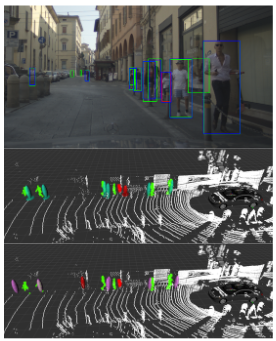
\includegraphics[width=0.4\linewidth]{Figures/Datasets/ECP_Dataset}
	\caption{This image shows an example of how the \gls{ECP2.5D} \cite{braun2020ecp2} dataset contains camera and LiDAR data in which pedestrians are annotated.}  
	\label{fig:dat_ecp}
\end{figure}

The \gls{BDD100K} dataset \cite{yu2020bdd100k} is collected using crowd-sourcing. Drivers could upload their data obtained by using a 1280x720 resolution front camera at 30 Hz together with GPS/IMU localization data. Recordings were mostly made in San Francisco and the Bay Area, New York, and Berkeley which makes it average on geographic diversity. Because of the crowd-sourcing, large amounts of data could be obtained. The dataset contains 100K 40-second sequences which makes it one of the largest datasets compared to the other datasets. Moreover, the dataset contains pixel-level semantic segmentation of the vehicle's drivable area. A downside of this dataset is that it is obtained using solely a monocular camera. Therefore, some unsupervised depth estimation technique must be performed to gather 3D data, like the \gls{STIP} dataset \cite{liu2020spatiotemporal}. \\

The \gls{KITTI} dataset \cite{geiger2012we} is the smallest dataset (of which the number of sequences is known) compared to the other datasets. It only contains 22 sequences and is obtained in only one country. The benefit of using this dataset is that it has been used by \cite{itkina2019dynamic}, \cite{mohajerin2019multi}, and \cite{lange2020attention} to generate and predict \glspl{OGM}. So, there is enough research to compare prediction methods with that use the \gls{KITTI} dataset \cite{geiger2012we}. \\

For the nuScenes dataset \cite{caesar2020nuscenes}, a LiDAR that can generate a 1.4M point 360 degree view at 20 Hz, five radars around the vehicle with a 250m range at 13 Hz, and six 1600x900 resolution cameras around the vehicle at 12 Hz are used to collect data. However, the sampling frequency of the data is only 2 Hz. This is the lowest sampling frequency compared to other datasets. Figure \ref{fig:dat_nuscenes} shows an example of the six camera images overlayed with the LiDAR point cloud of the nuScenes dataset \cite{caesar2020nuscenes}. The advantage of this dataset is that it contains velocity information from the radar data. Besides that, the nuScenes dataset is collected for object detection as well as object tracking. Therefore, it contains 1000 sequences of 20 seconds. Objects of 23 classes are annotated, including vehicles, pedestrians, and riders. So, the nuScenes dataset \cite{caesar2020nuscenes} is larger and more diverse than most other datasets. The nuScenes paper \cite{caesar2020nuscenes} compares its dataset against the \gls{KITTI} dataset \cite{geiger2012we}. It concludes that training on the \gls{KITTI} dataset, with its smaller size compared to nuScenes, affects a network's performance. \\

\begin{figure}[h!]
	\centering
	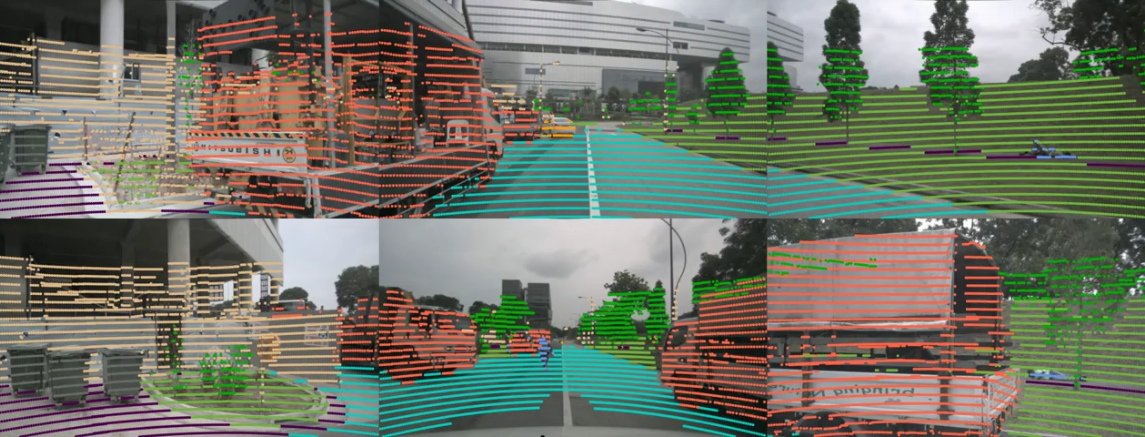
\includegraphics[width=0.6\linewidth]{Figures/Datasets/NuScenes_Dataset}
	\caption{This image shows an example of the images of the six cameras from the nuScenes dataset \cite{caesar2020nuscenes}. The images are overlayed with the semantic segmented LiDAR data.}  
	\label{fig:dat_nuscenes}
\end{figure}

The Waymo Open dataset - Perception - \cite{sun2020scalability} (in short Waymo), was originally recorded in 3 cities (Phoenix, San Francisco, and Mountain View) and later extended with another 3 cities (Los Angeles, Detroit, and Seattle). This makes the dataset average on geographic diversity. It contains 1150 20 second sequences at 10 Hz. It contains 10.8M objects with tracking IDs, labels for four object classes (vehicles, pedestrians, cyclists, and signs), and 3D bounding boxes of each of those objects. Moreover, \cite{lange2020attention} and \cite{toyungyernsub2020double} used the Waymo dataset to generate and predict \glspl{OGM}, so there is research to compare prediction methods with using the Waymo dataset \cite{sun2020scalability}.


\subsection{Semantic Segmentation Datasets} \label{subsec:data_sem_seg}
This section discusses two datasets that are originally generated for semantic segementation tasks. The Apolloscape dataset \cite{huang2019apolloscape}  and the Cityscapes dataset \cite{cordts2016cityscapes}. \\

Apolloscape \cite{huang2019apolloscape} is a dataset which is collected for the purpose of scene parsing (semantic segmentation on pixel-level). Therefore, the dataset contains almost 144K frames with pixel-level annotations for semantic segmentation. Furthermore, 89K instance-level annotations are provided for movable objects. 25 different labels are annotated covering five groups. Also, 28 lane markings are annotated. Together there are 543K pedestrian instances and 1.99M vehicle instances in the dataset. This makes the dataset diverse regarding traffic participants. The downside is that the dataset is recorded in only one city, and there is no information available about presence of sequences (only individual frames). \\

\begin{figure}[h!]
	\centering
	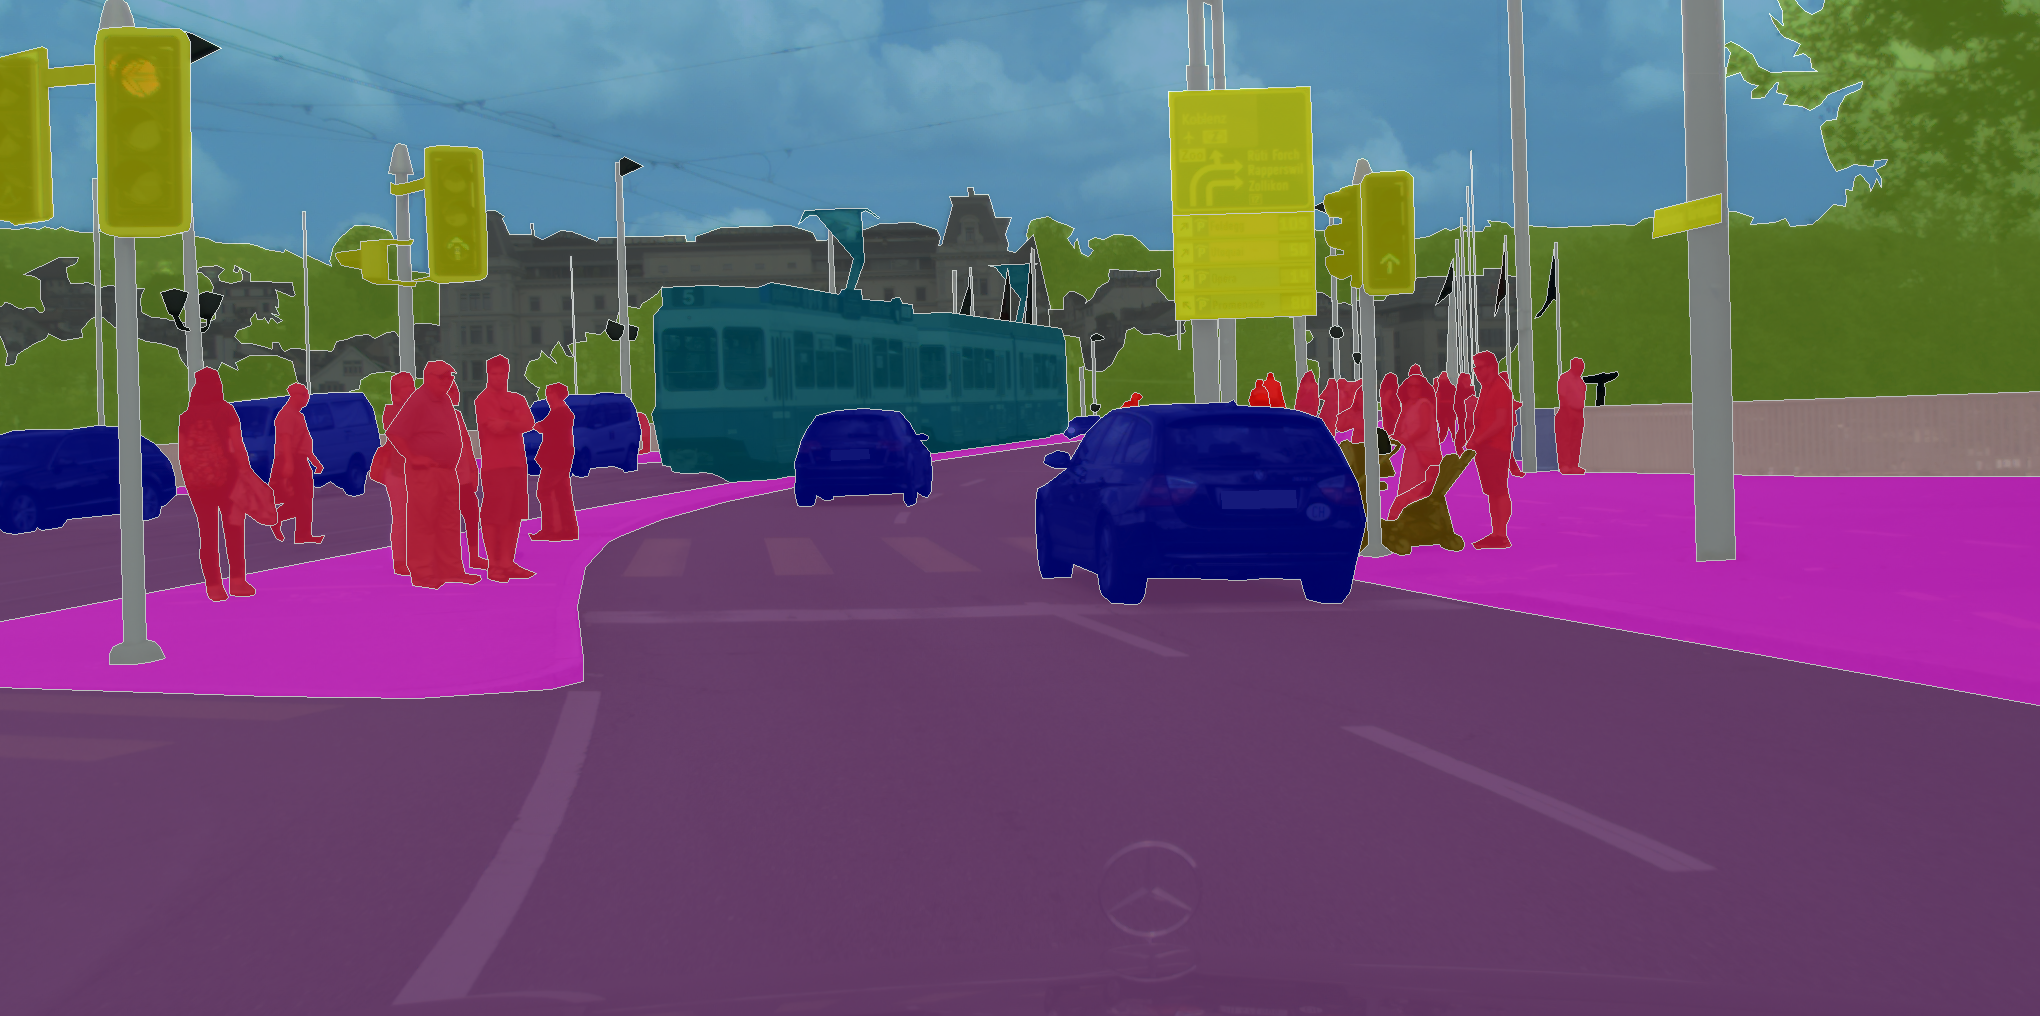
\includegraphics[width=0.6\linewidth]{Figures/Datasets/Cityscapes_Dataset}
	\caption{This image shows an example of the Cityscapes \cite{cordts2016cityscapes} dataset. The camera image is semantically segmented. Each object class in the image is given a different label (color).}  
	\label{fig:dat_cityscapes}
\end{figure}

The Cityscapes dataset \cite{cordts2016cityscapes} is recorded in 50 different cities, primarily in Germany but also in neighboring countries. From 27 cities, 5000 images are selected for dense pixel-level annotation. Annotations are done on every 20th frame of a 30-frame video sequence. For the remaining 23 cities, coarse annotation is performed on a single image every 20 seconds or 20 meters driving distance (whichever comes first). This yields another 20K annotated images. An example an annotated image from the dataset is shown in figure \ref{fig:dat_cityscapes}. 30 classes are annotated which are grouped into 8 categories. The dataset contains 24.4K annotated pedestrians and 41K vehicles. Humans and vehicles are also annotated on an instance level. Therefore, this dataset is diverse regarding both geographic locations and traffic participants. The dataset has also been used to generate \glspl{OGM} by \cite{hehn2021fast}. The downside of this dataset is that the number of sequences is not known, besides that it is a 'large set'. 

\subsection{What dataset is most suitable to generate \gls{OGM} sequences for \gls{OGM} prediction?} \label{subsec:data_con}

Table \ref{tab:datasets_overview} shows an overview of the datasets that are discussed in the previous subsections. Based on the properties of each dataset it is evaluated how well they meet the criteria that were set at the beginning of this chapter. If a criterion is met, the score of the dataset goes up by 1 point. If the criterion is met partially, or in average quality compared to the other datasets, the score goes up by 0.5 point. If a criterion is not met, or if it is met in a bad quality compared to other datasets, the dataset will not get any points for that criterion. Also, if information about a criterion is not found or not available, no points are given to the criterion. Table \ref{tab:datasets_criteria} shows an overview of how well each datasets scores per criterion. More information about the symbols and what score is linked to them is written below the table. \\

\begin{figure}[h]
	\centering
	\begin{subfigure}[t]{0.4\linewidth}
		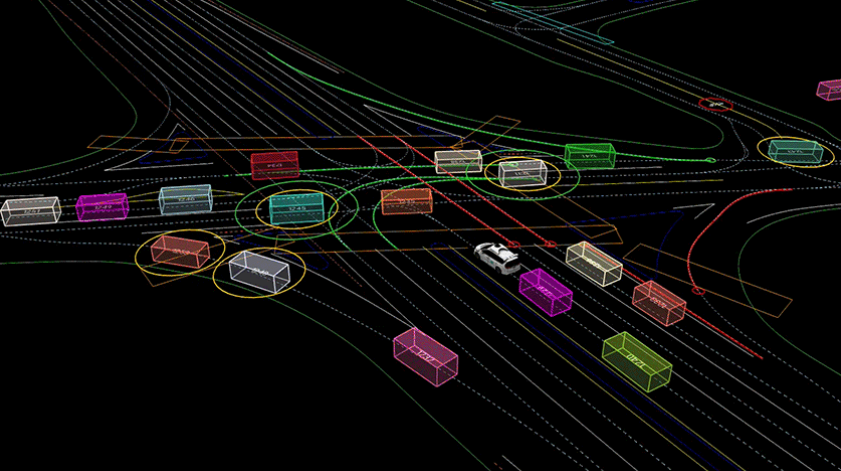
\includegraphics[width=\linewidth]{Figures/Datasets/Waymo_Dataset}
		\caption{This image shows an overview of the labeled vehicles and lane markings of the Waymo \cite{sun2020scalability} dataset.}
		\label{fig:dat_waymo_1}
	\end{subfigure} \hspace{0.1\textwidth}
	\begin{subfigure}[t]{0.4\linewidth}
		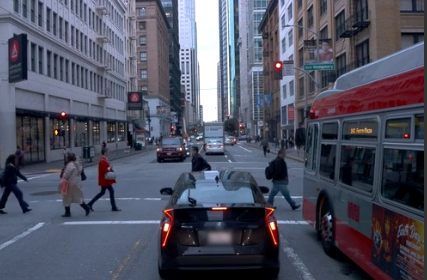
\includegraphics[width=\linewidth]{Figures/Datasets/Waymo_Dataset2}
		\caption{This image shows a front camera image of the Waymo \cite{sun2020scalability} dataset.}
		\label{fig:dat_waymo_2}
	\end{subfigure}
	\caption{Two examples of the Waymo \cite{sun2020scalability} dataset.}
	\label{fig:dat_waymo_both}
\end{figure}

With a score of 7.5, the Waymo \cite{sun2020scalability} dataset (shown in figure \ref{fig:dat_waymo_both}) is the most suitable dataset to generate \gls{OGM} sequences for \gls{OGM} prediction. While the diversity of the Waymo dataset is average, compared to the other datasets, and there is no (available) data to extend the \gls{OGM} form, the Waymo dataset meets all other criteria in good quality which sums up to the score of 7.5. Other suitable datasets on the second and shared third places are the Cityscapes \cite{cordts2016cityscapes}, Argoverse \cite{chang2019argoverse} and NuScenes \cite{caesar2020nuscenes} datasets with a score of 7.0, 6.5 and 6.5 respectively. Unlike the Waymo dataset, the Cityscapes dataset provides pixel-level semantic segmentation data and the Nuscenes dataset provides velocity data and semantic LiDAR data. In the case this additional data is desired for research on a specific \gls{OGM} prediction method, the Cityscapes or Nuscenes datasets can be more suitable to use than the Waymo dataset. Also, conveniently, for the four best scoring datasets there is literature available that provides code to generate \glspl{OGM} from the data. These sources can be found in table \ref{tab:datasets_overview}.  

\afterpage{%
	\clearpage% Flush earlier floats (otherwise order might not be correct)
	\thispagestyle{empty}% empty page style (?)
	\begin{landscape}
\begin{table}[h!]
	\centering
	\resizebox{\linewidth}{!}{%
		\begin{tabular}{lllllllllll} 
			\toprule
			& \textbf{STIP \cite{liu2020spatiotemporal}} & \textbf{Argoverse \cite{chang2019argoverse}} & \textbf{ECP2.5D \cite{braun2020ecp2}} & \textbf{BDDK100 \cite{yu2020bdd100k}} & \textbf{KITTI \cite{geiger2012we}} & \textbf{NuScenes \cite{caesar2020nuscenes}} & \textbf{Waymo \cite{sun2020scalability}} & \textbf{Apolloscape \cite{huang2019apolloscape}} & \textbf{Cityscapes \cite{cordts2016cityscapes}} & \textbf{RobotCar \cite{robotcardatasetijrr}} \\ 
			\hline
			\textbf{1} & \xmark & \cmark & \cmark & \xmark & \cmark & \cmark & \cmark & \cmark & \cmark & \cmark \\
			\textbf{2} & \textbf{$\pm$} & \textbf{$\pm$} & \textbf{$\pm$} & \textbf{+} & \textbf{$-$} & \textbf{$\pm$} & \textbf{$\pm$} & \textbf{$-$} & \textbf{+} & \textbf{$-$} \\
			\textbf{3} & \textbf{$\pm$} & \textbf{+} & \textbf{$\pm$} & \textbf{+} & \textbf{$-$} & \textbf{+} & \textbf{+} & U & U & U \\
			\textbf{4} & \textbf{+} & \textbf{+} & \textbf{+} & U & \textbf{+} & \textbf{$-$} & \textbf{+} & U & \textbf{+} & \textbf{+} \\
			\textbf{5} & \cmark & \cmark & \cmark & \cmark & \cmark & \cmark & \cmark & \cmark & \cmark & U \\
			\textbf{6} & \cmark & \cmark & \cmark & \cmark & \cmark & \cmark & \cmark & \cmark & \cmark & \cmark \\
			\textbf{7} & \textbf{$\pm$} & \textbf{$\pm$} & \textbf{$\pm$} & \textbf{$\pm$} & \textbf{$\pm$} & \textbf{$\pm$} & \textbf{+} & \textbf{$\pm$} & \textbf{$\pm$} & \textbf{$\pm$} \\
			\textbf{8} & N & N & N & Pixel Semantics & N & Velocity data, LiDAR Semantics & N & Pixel Semantics & Pixel Semantics & N \\
			\textbf{9} & N & Only OGM gen & N & N & OGM gen and pred & Only OGM gen & OGM gen and pred & N & Only OGM gen & OGM gen and pred \\
			\textbf{Scores} & 4.5 & \textbf{6.5} & 5.5 & 5.5 & 5.5 & \textbf{6.5} & \textbf{7.5} & 4.5 & \textbf{7.0} & 4.5 \\
			\bottomrule
		\end{tabular}
	}
	\caption{
		The table shows for each dataset how well it scores per criterion. The scores are based on the information in table \ref{tab:datasets_overview}. The following symbols are used to evaluate each criterion: 
		\textbf{+:} Good, \textbf{$\pm$:} Average, \textbf{$-$:} Bad, \textbf{U:} Unknown: \textbf{N:} None/Not available/Not found, \textbf{\cmark:} Yes, \textbf{\xmark:} No. \\\hspace{\textwidth} 
		At the bottom row, each dataset is given a score based on which symbol is given at the evaluation, and whether there is useful information found for criteria 8 and 9. A '\textbf{+}', a '\textbf{\cmark}', 'OGM gen and pred', and any available additional data for an extended OGM form provide 1 point, an '\textbf{$\pm$}' and 'only OGM gen' provides 0.5 points, and the '\textbf{\xmark}', '\textbf{$-$}', 'U', and 'N' provide 0 points.  
		Below is the list of criteria. \\\hspace{\textwidth} 	
		\textbf{1.} The dataset contains data of ego-vehicle centered traffic scene sequences that provide at least 2D \gls{BEV} information of the environment.
		\textbf{2.} The dataset provides enough diverse data to train and evaluate a network on.
		\textbf{3.} The dataset contains traffic scene sequences, or provides means to easily generate them.
		\textbf{4.} The sequences have enough frames per sequence and a frame frequency that is suitable for capturing road user behavior and trajectories.
		\textbf{5.} The sequences contain various traffic actors including vehicles and \glspl{VRU}.
		\textbf{6.} The dataset data, and any \glspl{OGM} that can be generated from it, provides a resolution that is high enough to distinguish and to track \glspl{VRU}. 
		\textbf{7.} The sequences show a diversity in environmental properties, containing \glspl{VRU}, that may influence the generated \glspl{OGM} (e.g. urban vs rural, dense vs sparse traffic).
		\textbf{8.} The dataset provides data, including ground truth, that is required for generating extended \gls{OGM} forms.
		\textbf{9.} Results of other research using the dataset for generating and predicting \glspl{OGM} is available for comparison.}
	\label{tab:datasets_criteria}
\end{table}
	\end{landscape}
}

%%

\afterpage{%
	\clearpage% Flush earlier floats (otherwise order might not be correct)
	\thispagestyle{empty}% empty page style (?)
	\begin{landscape}
		\begin{longtable}{m{4em}m{2em}m{7em}m{7em}m{5em}m{2em}m{5em}m{7em}m{4em}m{2em}m{2em}m{5em}m{1em}m{1em}} 
			\toprule
			\rotatebox{90}{\textbf{Dataset}} & \rotatebox{90}{\textbf{Year}} & \multicolumn{3}{c}{\rotatebox{90}{\textbf{Sensors}}} & \rotatebox{90}{\textbf{Sampling Frequency}} & \rotatebox{90}{\textbf{Diversity of Locations}} & \rotatebox{90}{\textbf{Dataset size}} & \rotatebox{90}{\textbf{Diversity of labels}} & \rotatebox{90}{\textbf{\# Pedestrians}} & \rotatebox{90}{\textbf{\# Vehicles}} & \rotatebox{90}{\textbf{Extended OGMs}} & \rotatebox{90}{\textbf{OGM generation method}} & \rotatebox{90}{\textbf{OGM prediction comparison}} \endfirsthead
			\midrule
			\textbf{STIP \cite{liu2020spatiotemporal}} & 2020 & - & 3 RGB cameras of res 1216x1936  (20 Hz) & - & 20 Hz & 1 country, 8 cities, dense urban areas & 556 sequences, \textasciitilde{}2h of recording, \textasciitilde{}150K frames & 2 classes (pedestrian, vehicle) & \textasciitilde{}3K & - & - & - & - \\
			\textbf{Argoverse \cite{chang2019argoverse}} & 2019 & 2 VLP-32 LiDARs with 200m range (10 Hz) & 7 RGB cameras in 360 deg setup of res 1920x1200 (30 Hz) and 2 in stereo view of res  2056x2464 (5 Hz) & GPS/ Odometry sensor & 10 Hz & 1 country, 2 cities, dense urban areas & \textasciitilde{}333K 5s sequences, 1006h of recording, spanning \textasciitilde{}290km & 17 classes & \textasciitilde{}1.5K & \textasciitilde{}8K & - & \cite{roddick2020predicting} & - \\
			\textbf{ECP2.5D \cite{braun2020ecp2}} & 2020 & Velodyne HDL-64E LiDAR with 120m range (5-20 Hz) & 1 RGB camera of res 1920x1024 (20 Hz) & GPS/INS & 20 Hz & 12 countries, 31 cities, dense urban areas & 15s sequences, 46K frames & 7 classes & \textasciitilde{}218K & - & - & - & - \\
			\textbf{BDDK100 \cite{yu2020bdd100k}} & 2020 & - & 1 camera of res 1280x720 (30 Hz) & GPS/IMU & - & (mostly) 1 country, 4 cities, dense urban areas & \textasciitilde{}100K 40s sequences & 3 categories, 20 classes & \textasciitilde{}129K & \textasciitilde{}1M & Pixel-level semantic segmentation & - & - \\
			\textbf{KITTI \cite{geiger2012we}} & 2012 & Velodyne HDL-64 LiDAR with 100m range (10 Hz) & 4 cameras (2 color 2 grayscale) of res 1392x512 (10 Hz) & GPS/IMU & 10 Hz & 1 country, 1 city, dense urban areas & 22 sequences & 2 categories, 8 classes & \textasciitilde{}9.4K & \textasciitilde{}100K & - & \cite{itkina2019dynamic} \cite{mohajerin2019multi} \cite{lange2020attention} & \cite{itkina2019dynamic} \cite{mohajerin2019multi} \cite{lange2020attention} \\
			\textbf{NuScenes \cite{caesar2020nuscenes}} & 2019 & 32 beam LiDAR 1.4M points/s (20 Hz) + 5 Radars with 250m range (13 Hz) & 6 cameras of res 1600x900 cameras (12 Hz) & GPS/IMU, CAN bus data & 2 Hz & 2 countries, 2 cities, dense urban areas & 1000 20s sequences & 23 classes, 8 attributes & \textasciitilde{}200K & \textasciitilde{}500K & velocity information from Radar with 0.1km/h accuracy and LiDAR semantics & \cite{roddick2020predicting} \cite{loukkal2021driving} & - \\
			\textbf{Waymo \cite{sun2020scalability}} & 2020 & 5 LiDAR sensors (1 mid range, 4 short range) & 5 cameras (3 front of res 1920x1280 and 2 side of res 1920x1014) & - & 10 Hz & 1 country, 6 cities, urban and suburban areas & 1150 20s sequences & 3 classes & \textasciitilde{}2.8M & \textasciitilde{}6.1M & - & \cite{lange2020attention} \cite{toyungyernsub2020double} & \cite{lange2020attention} \cite{toyungyernsub2020double} \\
			\textbf{Apolloscape \cite{huang2019apolloscape}} & 2018 & 2 VUX-1HA LiDARs with 420m range & 1 VMX-CS6 camera system with 2 cameras of res 3384x2710 (no depth information) & IMU/GNSS & - & 1 country, dense urban areas & - & 5 categories, 35 classes, additional 28 kinds of lane markings & \textasciitilde{}543K & \textasciitilde{}1.99M & Pixel-level semantic segmentation & - & - \\
			\textbf{Cityscapes \cite{cordts2016cityscapes}} & 2020 & - & 1 stereo camera of res 1920x1080 (OnSemi AR0331) (17 Hz) & GPS, outside temperature, in-vehicle odometry sensors & 17 Hz & 1 country, 50 cities, dense urban areas & A 'large set' of sequences & 8 categories, 30 classes & \textasciitilde{}24.4K & \textasciitilde{}41K & Pixel-level semantic segmentation & \cite{hehn2021fast} & - \\
			\textbf{RobotCar \cite{robotcardatasetijrr}} & 2016 & 2 SICK LMS-151 2D LiDARs with 50m range (50 Hz) and 1 SICK LD-MRS 3D LiDAR with 50m range (12.5 Hz) & 4 cameras (1 front of res 1280x960 at 16 Hz, 3 for sides and rear of res 1024x1024 at 11.1 Hz) & GPS/INS & - & 1 country, 1 city, urban area & 360s sequences of unknown amount & No labels & - & - & - & \cite{dequaire2018deep} \cite{wang2020l2r} & \cite{dequaire2018deep} \\
			\bottomrule
		\caption{This table shows an overview of the datasets that are most likely to be suitable for \gls{OGM} prediction purposes.}
		\label{tab:datasets_overview}	
		\end{longtable}	
	\end{landscape}
}

%%


\newpage

\section{Metrics} \label{sec:metrics}

\glspl{AV} can have collision avoidance systems that make use of traffic scene predictions to estimate whether the ego-vehicle will collide with any of the surrounding traffic participants. Based on these systems the \gls{AV} can make decisions to drive as safe as possible by preventing or mitigating collisions. For example, if a collision is predicted, the ego-vehicle can decide to adjust its velocity to prevent or mitigate the collision, or it will decide to perform an evasive maneuver \cite{annell2016probabilistic} \cite{wang2019crash}. \cite{annell2016probabilistic}'s system has even shown to be robust to noise in the environment representation. However, due to prediction errors, such as artifacts or displacement errors of traffic participants, the \gls{AV} might make the wrong decisions (e.g. perform an evasive maneuver when in reality there is no imminent collision, or fail to perform an evasive maneuver when there is actually a collision risk). This can be dangerous for the \gls{AV} and its surroundings. Besides for the task of collision avoidance, prediction of an \gls{AV}'s surroundings can also improve the efficiency and safety of motion planning by \glspl{AV} in general. Ensuring safe motion planning means that no (additional) dangerous situations are caused when the \gls{AV} executes a path that is planned in the \gls{OGM} predictions, compared to a path that is planned in the ground truth \gls{OGM}. So, for the safety of \glspl{AV} and its surroundings, good predictions are important. Since this literature study focuses on \gls{OGM} predictions, a metric is desired that compares the predicted \glspl{OGM} with the ground truth \glspl{OGM}. \\

The quantitative evaluation of \gls{OGM} prediction methods depends highly on what metric is used to assess a method's performance. The metric determines which errors are considered and how much they weigh in the evaluation. What the best metric is for \gls{OGM} prediction is therefore investigated in this chapter.
However, there is (almost) no literature on what properties constitute a good metric for \gls{OGM} prediction methods. What literature stresses, is that the (predictive) systems in \glspl{AV} must improve the safety of traffic and ensure safe behavior of the \gls{AV}. Safe behavior consists of avoiding or mitigating collisions \cite{kaempchen2009situation} \cite{annell2016probabilistic}. To execute this safe behavior, the \gls{AV} must accurately sense or predict its environment \cite{mitra2018towards} \cite{themann2015impact} \cite{annell2016probabilistic}. From this reasoning, one can state that \gls{OGM} predictions must be evaluated based on their accuracy of the environment representation and the safety of the \gls{AV}'s behavior that results from the them. \cite{gandhi2007pedestrian} states that it is important to evaluate pedestrian protection systems that ensure safety, such as pedestrian collision prediction, using standardized performance metrics. However, no metric criteria are mentioned which constitute a good metric. Because of the lack of literature about metric criteria for \gls{OGM} prediction, this literature review devises the criteria based on the assurance of traffic safety. \\

To ensure safety, a metric is desired to meet the following demands. The more similar a prediction is to the ground truth, the better the metric should score the prediction. Also, global errors such as noise do not affect robust \gls{AV} motion planning systems. Therefore, global errors should be weighed less in the metric score than local errors, such as artifacts or displacement errors. Then, prediction errors that are more likely to cause the \gls{AV} to perform dangerous maneuvers, should have a worse score compared to prediction errors that are likely harmless. Furthermore, \glspl{AV} have less time to correct their paths when there are large displacement errors or errors close to the \gls{AV}. So, these errors should be considered worse than small displacement errors or errors further from the \gls{AV}. Moreover, if there are artifacts, deletions or additions of occupied clusters, in the predictions, the \gls{AV} might perform dangerous confronting or evasive maneuvers respectively. Therefore, deletions and additions should be penalized more than displacements. These demands result in the following list of criteria that a metric must meet in order to evaluate an \gls{OGM} method that ensures that safer predictions are considered better.

\begin{enumerate}
	\item The metric considers the whole \gls{OGM} in its evaluation.
	\item The metric weighs local errors more than global errors.
	\item The metric weighs big displacement errors more than small displacement errors. 
	\item The metric weighs errors close to the \gls{AV} (often the center of the \gls{OGM}) more than errors further from the \gls{AV}.
	\item The metric weighs additions and deletions more than displacements.
\end{enumerate}

A selection of five metrics that are used to measure the quality of \glspl{OGM} compared to the ground truth is made based on papers that research \gls{OGM} prediction methods. These metrics are evaluated in this section based on the criteria described in this chapter. First, the \glsfirst{MSE} is evaluated in section \ref{subsec:mse_met}. Second, the \glsfirst{SSIM} is evaluated in section \ref{subsec:ssim_met}. Third, section \ref{subsec:is_met} evaluates the \glsfirst{IS} metric. Fourth, secion \ref{subsec:froc_met} evaluates the F1 score and \glsfirst{ROC} metrics together, because those metrics are based on similar mathematical principles. Finally, section \ref{subsec:con_met} answers the sub-question: \airquote{\textit{What is the best quantitative metric to determine the accuracy of a predicted OGM?}}

\subsection{\glsfirst{MSE}} \label{subsec:mse_met}
The \glsfirst{MSE} metric is used by \cite{itkina2019dynamic}, \cite{lange2020attention}, and \cite{toyungyernsub2020double} to compare the \gls{OGM} predictions with the ground truth. \cite{lange2020attention} and \cite{toyungyernsub2020double} also use the \glsfirst{IS} metric which is discussed later in this chapter. The \gls{MSE} metric formula is shown in equation \ref{eq:mse}, where $Y$ is an $m \times n$ \gls{OGM}, $X$ its prediction, and $i$ and $j$ the \gls{OGM} coordinates.

\begin{equation} \label{eq:mse}
	MSE = \frac{1}{mn}\sum_{i=0}^{m-1}\sum_{j=0}^{n-1}[Y(i,j)-X(i,j)]^2
\end{equation}

The equation evaluates the predicted \gls{OGM} as a whole and sums up the square of each cell's difference in value compared to the ground truth. So, the higher \gls{MSE}, the more its cell's values differ from the ground truth on a global scale. \cite{toyungyernsub2020double}'s research shows that the \gls{MSE} increases with the prediction time horizon of the \gls{OGM}, which is expected because of the accumulation of prediction errors with every time step. Because of its simplicity, the \gls{MSE} is used to assess not only \glspl{OGM} but images in general. However, there are implicit assumptions when using the \gls{MSE} \cite{wang2009mean}. The main assumptions are that the \gls{MSE} treats spatial positions of the grid cells, the sign of the error, and the relationship between the prediction and the ground truth independently, while it treats each cell with equal importance. Therefore, the \gls{MSE} cannot recognize relations within an \gls{OGM}, consider context, or differentiate local errors from global errors. The \gls{MSE} would thus not be able to assess displacements, deletions or additions. It is, however, possible to give errors close to the \gls{OGM}'s center a higher weighting by multiplying those errors by a penalty factor.    

\subsection{\glsfirst{SSIM}} \label{subsec:ssim_met}
The \gls{SSIM} is used by \cite{mohajerin2019multi} to evaluate the predicted \glspl{OGM} in their research. The \gls{SSIM} is based on the underlying principle "that the human visual system is highly adapted to extract structural information from visual scenes." \cite{wang2009mean}. This principle makes humans sensitive in identifying structural distortions in images, which is the reason that the \gls{SSIM} is designed to simulate that principle by focusing on image structure. Besides being sensitive for structural distortions, the human visual system also naturally compensates for non-structural distortions such as luminance (brightness) and contrast, since natural lighting causes a large variability in these distortions. The influence of luminance and contrast is separated from the structural distortions for better visual comprehension and recognition. The \gls{SSIM} task is therefore subdivided into three comparisons: luminance, contrast, and structure \cite{wang2004image}. These parts are explained as follows.\\

First the luminance of the \gls{OGM} is computed. The luminance is assumed to be the mean intensity of an \gls{OGM}. Equation \ref{eq:ssim_lumin} shows the formula for computing the luminance $\mu_X$, where $m \times n$ is the size of the \gls{OGM} and $X$ represents an \gls{OGM}. The luminance value of the ground truth and the prediction are compared using equation \ref{eq:ssim_lumin_compare}, where $X$ and $Y$ represent the predicted \gls{OGM} and ground truth respectively and $C_1 = (K_1 L)^2$, where $L$ is the dynamic range of the pixel intensity values (255 for 8-bit grids), and $K_1 \ll 1$ is a small constant.

\begin{equation} \label{eq:ssim_lumin}
	\mu_X = \frac{1}{mn}\sum_{i=0}^{m-1}\sum_{j=0}^{n-1}X_i(i,j)
\end{equation}
\begin{equation} \label{eq:ssim_lumin_compare}
	l(X,Y) = \frac{2\mu_X \mu_Y + C_1}{\mu_X ^2 + \mu_Y ^2 + C_1}
\end{equation}

Second, the \gls{OGM}'s contrast is computed. The contrast ratio is assumed to be the standard deviation $\sigma_X$ of the \gls{OGM}, shown in equation \ref{eq:ssim_contrast}. The contrasts of the prediction and the ground truth are then compared using equation \ref{eq:ssim_contrast_compare}, where $C_2 = (K_2 L)^2$, $L$ is the dynamic range of the pixel intensity values, and $K_2 \ll 1$ is a small constant.

\begin{equation} \label{eq:ssim_contrast}
	\sigma_X = \left(\frac{1}{mn-1}\sum_{i=0}^{m-1}\sum_{j=0}^{n-1}(X(i,j) - \mu_X)^2 \right)^\frac{1}{2}
\end{equation}
\begin{equation} \label{eq:ssim_contrast_compare}
	c(X,Y) = \frac{2\sigma_X \sigma_Y + C_2}{\sigma_X ^2 + \sigma_Y ^2 + C_2}
\end{equation}

Third, equation \ref{eq:ssim_structure_compare} is used to compare the structures between the prediction and the ground truth, where $C_3$ is a small constant and $\sigma_{XY}$ is computed using equation \ref{eq:ssim_structure_sig}.

\begin{equation} \label{eq:ssim_structure_compare}
	s(X,Y) = \frac{\sigma_{XY}+C_3}{\sigma_X\sigma_Y+C_3}
\end{equation}
\begin{equation} \label{eq:ssim_structure_sig}
	\sigma_{XY} = \frac{1}{mn-1}\sum_{i=0}^{m-1}\sum_{j=0}^{n-1}(X(i,j)-\mu_X)(Y(i,j) -\mu_Y)
\end{equation}

After the comparisons are performed, the \gls{SSIM} combines them according to equation \ref{eq:ssim}, "where $\alpha > 0$, $\beta > 0$ and $\gamma > 0$ are parameters used to adjust the relative importance of the three components." \cite{wang2004image}. For simplicity, these values can be set as $\alpha = \beta = \gamma = 1$ and $C_3 = C_2/2$ \cite{wang2004image}. The \gls{SSIM} ranges from $0$ to $1$, where $0$ means that the evaluated image is completely different from the ground truth, while a value of $1$ means that the evaluated image is identical to the ground truth.

\begin{equation} \label{eq:ssim}
	SSIM(x,y) = [l(x,y)]^\alpha \cdot [c(x,y)]^\beta \cdot [s(x,y)]^\gamma
\end{equation}

The \gls{SSIM} has the beneficial property that it can be used globally as well as locally (by separately evaluating spatial sections of an \gls{OGM}). Also, because the \gls{SSIM} is focused on structural similarities, it is expected that small displacements are weighed less than large displacement, and that displacements are weighed less than additions or deletions, since displacements retain the original structure, while the additions and deletions disrupt the original structure. Finally, similarly to the \gls{MSE}, the \gls{SSIM} can give a higher weighting to errors in the center of an \gls{OGM} if it is subdivided into sections and the center sections are given a higher error penalty.


\subsection{\glsfirst{IS}} \label{subsec:is_met}
The \glsfirst{IS} metric is used in \cite{lange2020attention} and \cite{toyungyernsub2020double} to measure the predictions' quality of the scene structure compared to the ground truth. \cite{birk1996learning} developed the \gls{IS} metric which they later used in \cite{birk2006merging}'s research on finding similarities between \glspl{OGM} in order to merge them to generate bigger maps. \cite{birk1996learning} defines the \gls{IS} metrics according to  equations \ref{eq:is_met} and \ref{eq:is_met_dist}.


\begin{equation} \label{eq:is_met}
	IS(m_1, m_2) = \sum_{c \in C}^{}d(m_1, m_2,c) + d(m_2,m_1,c)
\end{equation}

\begin{equation} \label{eq:is_met_dist}
	d(m_1, m_2,c) = \frac{\sum_{m_1[p_1]=c}^{} min\{md(p_1, p_2)|m_2[p_2]=c\}}{\#_c(m_1)}
\end{equation}

Where $C$ denotes the set of 'colors', in the case of an \gls{OGM} empty, unknown and occupied. $m_i[p]$ is the color $c$ of grid $m_i$ at position $p=(x,y)$. $md(p_1,p_2) = |x_1 - x_2| + |y_1 - y_2|$ is the Manhattan-distance between $p_1$ and $p_2$. $\#_c(m_i) = \#{p_1|m_i[p_1] = c}$ is the number of pixels in $m_i$ with color $c$ \cite{birk1996learning}. \\
The \gls{IS} metric is the sum over all the grids colors (grid cell states) of the average Manhattan-distance of the cells with color $c$ (i.e. empty, unknown or occupied) in grid map $m_i$ to the nearest cell with color $c$ in grid map $m_j$ ($d(m_1, m_2,c)$) and the average Manhattan-distance vice versa \cite{birk1996learning}. The higher the \gls{IS} value, the larger the difference between the evaluated image and the ground truth. \\

The \gls{IS} metric, similarly to the \gls{SSIM}, compares image structures. Therefore, this metric can be used both on a global and local (spatial subsections) scale to compare \glspl{OGM}. Also, because \gls{IS} metric evaluates based on structure, it is expected that small displacements are weighed less than large displacements, and displacements in general are weighed less than deletions and additions. Like the other metrics, higher weights can be given to spatial subsections that match the \gls{AV}'s location (center of the grid map) to weigh errors close to the \gls{AV} more than errors farther away from the \gls{AV}.

\subsection{F1 score and \glsfirst{ROC}-curve} \label{subsec:froc_met}
To evaluate \gls{OGM} prediction quality, \cite{dequaire2018deep} uses the F1 score (equation \ref{eq:f1score}), \cite{hoermann2018dynamic} the \gls{ROC}-curve, and \cite{schreiber2019long} uses both. These two metrics together make use of the \gls{TPR} (Recall) in equation \ref{eq:recall}, \gls{PPV} (Precision) in equation \ref{eq:precision}, and \gls{FPR} (Fall-out) in equation \ref{eq:fallout} to determine how well the predictions match the ground truth. Here, a positive condition signifies that a grid cell is occupied, where a negative condition signifies that it is empty.

\begin{equation} \label{eq:recall}
	recall = TPR = \frac{\sum True Positive}{\sum Condition Positive}
\end{equation}

\begin{equation} \label{eq:precision}
	precision = PPV = \frac{\sum True Positive}{\sum Predicted Condition Positive}
\end{equation}

\begin{equation} \label{eq:fallout}
	fall\text{-}out = FPR = \frac{\sum False Positive}{\sum Condition Negative}
\end{equation}

\begin{equation} \label{eq:f1score}
	F_1 = 2 \cdot \frac{precision \cdot recall}{precision + recall}
\end{equation}

The F1 score combines the precision (\gls{PPV}) and recall (\gls{TPR}) of a predicted \gls{OGM} to generate a score that is $1$ if the prediction is identical to the ground truth and $0$ if the prediction does not match the ground truth at all (meaning no true positives are predicted). The recall is the probability that a positive grid cell in the ground truth is also predicted as positive. Precision is the probability that a predicted positive grid cell is correctly predicted. \\

The \gls{ROC}-curve is a graphic metric in which the \gls{TPR} is plotted against the \gls{FPR} at various threshold values $\gamma$ for which a grid cell is considered occupied. When predicting \glspl{OGM}, it is desired that the \gls{TPR} is maximized and the \gls{FPR} is minimized. However, this performance depends partly on the threshold $\gamma$. If $\gamma = 0$, all grid cells with a value above $0$ are considered occupied (positive). This means that the \gls{TPR} is equal to $1$, but the \gls{FPR} is equal to $0$. The opposite happens when $\gamma = 1$. Those outcomes are not desired, so the optimal $\gamma$ is often found between $0$ and $1$.  \\

The F1 score and \gls{ROC}-curve evaluate an \gls{OGM} only on a global scale where each grid cell is regarded independently from other grid cells. Therefore, the metric does not distinguish large displacements from small ones or additions and deletions from displacements. It is possible to locally weigh some grid cells more than others if a penalty factor is implemented.



\subsection{What is the best quantitative metric to determine the accuracy of a predicted OGM?} \label{subsec:con_met}

The evaluation of the criteria which a metric must meet to be suitable for \gls{OGM} prediction is shown in table \ref{tab:metrics}. Based on this chapter's information about the different metrics, the most suitable metrics are the \gls{SSIM} and \gls{IS} metrics. These metrics meet all the criteria. However, to determine whether the \gls{SSIM} is more suitable than the \gls{IS} metric, or whether there is another metric that is more suitable than the metrics from this chapter, more research should be done to investigate \gls{OGM} evaluation metrics. 

\begin{table}
	\centering
	\resizebox{0.5\linewidth}{!}{%
		\begin{tabular}{lcccc} 
			\toprule
			& \textbf{\gls{MSE}} & \textbf{\gls{SSIM}} & \textbf{\gls{IS}} & \textbf{F1/\gls{ROC}} \\ 
			\midrule
			\textbf{1.} & \textbf{\cmark} & \textbf{\cmark} & \textbf{\cmark} & \textbf{\cmark} \\
			\textbf{2. } & \textbf{\xmark} & \textbf{\cmark} & \textbf{\cmark} & \textbf{\xmark} \\
			\textbf{3. } & \textbf{\xmark} & \textbf{\cmark} & \textbf{\cmark} & \textbf{\xmark} \\
			\textbf{4. } & \textbf{\cmark}& \textbf{\cmark} & \textbf{\cmark} & \textbf{\cmark} \\
			\textbf{5.} & \textbf{\xmark} & \textbf{\cmark} & \textbf{\cmark} & \textbf{\xmark} \\
			\bottomrule
		\end{tabular}
	}
	\caption{This table gives an overview of the metrics that can be used to evaluate \gls{OGM} predictions. For each criterion (numbers 1 to 5), the table shows whether the metric meets it (\textbf{\cmark}) or not (\textbf{\xmark}). The criteria are as follows. 
		\\\hspace{\textwidth} 
		\textbf{1.} The metric considers the whole \gls{OGM} in its evaluation.
		\textbf{2.} The metric weighs local errors more than global errors.
		\textbf{3.} The metric weighs big displacement errors more than small displacement errors. 
		\textbf{4.} The metric weighs errors close to the \gls{AV} (often the center of the \gls{OGM}) more than errors further from the \gls{AV}.
		\textbf{5.} The metric weighs additions and deletions more than displacements.
	}
	\label{tab:metrics}
\end{table}
% Also a part about loss functions? See Hoerman2020 Loss Functions

	\newpage
	%\section{Sequential input Deep Learning Networks} \label{sec:seqDLnets}

Prior knowledge about Deep Learning can be found here: 

\subsection{RNN}

RNN Encoder-Decoder: \cite{cho2014learning}

LSTM: \cite{hochreiter1997long}

GRU: \cite{cho2014properties}


\subsection{Sequential Convolutional Neural Networks}

Temporal Convolutional Network: \cite{lea2017temporal}

U-Net: \cite{ronneberger2015u}

Temporal Shift: \cite{lin2019tsm}	


\subsection{Transformer Networks}

Transformer: \cite{vaswani2017attention}


\subsection{What Deep Learning network is best to use for OGM prediction?}
	%\newpage
	\section{Prediction Methods using Occupancy Grid Maps} \label{sec:ogm_methods}

This chapter gives an overview of current motion prediction methods that utilize \glspl{OGM} as prior information for the predictions. A distinction is made between \gls{OGM} prediction methods and state prediction methods. The former are methods that predict the entire future environment in \gls{OGM} form (as described in the problem description in chapter \ref{sec:intro}). The latter are methods that predict either future centroids or future actor representations. Both methods do take \glspl{OGM} as input data. All described methods are deep learning based. First, four \gls{OGM} prediction methods are described, then two state prediction methods are described, followed by the answer to the final sub-question of this literature study: \textit{"What method generates the best \gls{OGM} predictions?"}

\subsection{Occupancy Grid Map Prediction Methods} 

%% PredNet progress
\subsubsection{PredNet based OGM predictors}

Itkina \cite{itkina2019dynamic} proposes to utilize Lotter's \cite{lotter2016deep} PredNet, which is an architecture that contains a Convolutional LSTM originally used for video prediction, to predict future occupancy grid map data based on past grid maps. This network is expected to be suitable for \glsfirst{OGM} prediction because an \gls{OGM} is similar to a frame in a video. \\


%% Can be removed or moved to OGM chapter %%
A grid map is an environmental representation that subdivides an area into single cells and estimates the states of each cell based on sensor data. Occupancy grid maps are a form of grid maps were each cell state is represented by its occupancy probability. \cite{nuss2014fusion}. These probabilities can be estimated with methods such as Bayes' inference or the Dempster-Shafer Theory \cite{dempster1968generalization}. For many robotics applications, including AVs, not only the occupancy state of its surroundings is of interest, but also the type of occupancy, such as its class. Nuss \cite{nuss2014fusion} proposed a method to fuse the class labeled information from camera images with the occupancy data from laser data to create occupancy grid maps with labeled objects.    
OGMs are a suitable environment representation for motion prediction because they can generate probabilistic maps without having data of the entire environment or making assumptions of agent behavior \cite{itkina2019dynamic}. \\
%% Can be removed or moved to OGM chapter %%

The convolutional layers are used to correlate the occupied cells in the grid map based on contextual information.
Itkina \cite{itkina2019dynamic} compares the PredNet's performance with a baseline that assumes a static environment (for the short period of time the predictions last), with a FCN network, and with a particle filter predictor. Itkina \cite{itkina2019dynamic} also compares the performance of the network with multiple variations of the input \glspl{OGM}. Using only static \glspl{OGM} is compared with using an additional Dynamic OGM (DOGMa), which includes an additional dimensional layer to the grid map that contains dynamic state information (e.g. velocity). Furthermore, the benefits of the Dempster-Shafer environment representation in the \glspl{OGM} is compared with using a probabilistic alternative. Comparisons are done qualitatively and with the MSE metric that compares each cell of the \glspl{OGM}. 

The research of Itkina \cite{itkina2019dynamic} found that the PredNet outperforms the other investigated methods. Also, the DST-based method performs better than the probability based method, and the difference in performance between the OGM and the DOGMa almost none. For longer predictions, the objects in the OGM become blurry or even disappear from the environment. 

To counter the blurriness and object disappearance for longer term predictions, Lange \cite{lange2020attention} proposes the Attention Augmented ConvLSTM (AAConvLSTM) for Environment Prediction. Lange \cite{lange2020attention} stresses the importance of OGM predictions, because this "approach facilitates the use of occupancy state estimation under uncertainty to update the belief of surroundings" \cite{lange2020attention}. However, the predictions must be reliable, so that is why Lange \cite{lange2020attention} tries to reduce blurriness by implementing an attention mechanism that originated from creating long-term dependencies in language processing into the PredNet architecture. Comparing the results with using the original PredNet architecture, the AAConvLSTM performs better both qualitatively and based on the MSE and Image Similarity (IS) metrics. However, blurriness and disappearance of objects remains.

Toyungyernsub \cite{toyungyernsub2020double} also attempts to counter the blurriness and disappearing objects that resulted from Itkina's \cite{itkina2019dynamic} method. They propose a double-prong ConvLSTM network based on the PredNet architecture which separately predicts the static and dynamic input \glspl{OGM} and fuses the results in a joined prediction of the OGM. The method outperforms the original PredNet both in terms of the IS and MSE metrics as qualitatively. The blurriness and disappearance of objects reduces significantly. For future work, incorporating multi-modality into the predictions is advised because the predicted object orientations were not always correct due to the variety of directions the objects could head for.

The networks of Itkina \cite{itkina2019dynamic}, Lange \cite{lange2020attention}, and Toyungyernsub \cite{toyungyernsub2020double} are trained on the KITTI \cite{geiger2013vision}, Waymo \cite{sun2020scalability} and KITTI \cite{geiger2013vision}, and Waymo \cite{sun2020scalability} datasets respectively.  

%% Hoerman
\subsubsection{Convolutional neural network based OGM predictors}
Hoermann \cite{hoermann2018dynamic}, proposes to predict Dynamic Occupancy Gridmaps (DOGMas) using a convolutional neural network. The network requires one DOGMa of the current timestep and predicts the future $0$ to $3$ seconds. It learns to label the objects, static or dynamic, to provide one static channel output and several dynamic channel outputs that together form an output DOGMa. Only one input DOGMA is used because it is hypothesized that most information necessary for prediction can be found in the dynamic representation and the relation between the cells and not necessarily from the past DOGMas. The paper argues that providing a DOGMa as output is beneficial because it is independent of the sensor setup since the network does not process the raw sensor data directly. Therefore, the network can be trained with varying sensors that provide the input DOGMas. Results show that the proposed method is better than a particle filter approach. The proposed method performs multimodal predictions, can distinguish static from dynamic objects, and provides more accurate predictions than the particle filter. This is because the convolutional layers capture the DOGMa's cell dependencies where particle filters assume independent cells. However, due to uncertainty longer term predictions become vaguer. 

Schreiber \cite{schreiber2019long} builds upon Hoermann's \cite{hoermann2018dynamic} research by expanding the convolutional neural network with an LSTM encoder and decoder, and skip connections with ConvLSTMs. Schreiber \cite{schreiber2019long} states that the prediction of future DOGMas is comparable to a video prediction problem due to the image-like structure of the DOGMas. The LSTMs are expected to exploit spatial and capture temporal correlations, while the skip connection ConvLSTMs are expected to handle missing data due to occlusion. Schreiber's \cite{schreiber2019long} method shows better F1-score results and better qualitative results compared to Hoermann's \cite{hoermann2018dynamic} previous research. The static predictions remain sharp for long term predictions, even for parts of the environment that became partially occluded in the input sequence. Partially occluded dynamic obstacles are predicted accurately as well and there is multimodality in the predictions. Communication signals and road signs are not taken into account. These cues could improve the (multimodal) predictions. Also, the data is only recorded in a stationary scenario, so the performance of the network with egomotion is not researched.   

%% Dequaire and Mohajerin
\subsubsection{Deep tracking based OGM predictors}
Dequaire's \cite{dequaire2018deep} research is based on end-to-end tracking of objects using \glspl{OGM} as environment representations. The research proposes a framework that learns a model of world dynamics in an unsupervised manner. The model can predict the unoccluded state, inluding occupancy, semantics, and dynamic behavior, of the world given a sequence of partially observable input OGMs. This partially observable sequence of the environment provides varying information about the objects that are present. The sequence is used as input for a GRU with dilated convolutional layers to track and classify the partially occluded objects. Dequaire \cite{dequaire2018deep} argues that predicting the future is the same as tracking and classifying the environment given partially occluded \glspl{OGM} of the past and 'future' OGMs that are completely occluded. The network will fill in the future occupancy in the completely occluded OGM based on the information from the past OGMs. Different network configurations' results are compared using the F1 measure and IoU to assess tracking performance and scene semantics quantitatively.  

Mohajerin \cite{mohajerin2019multi} reasons that having OGMs as output provides drivable space information without the need of several stages (detection, classification, tracking, predicting, occupancy grid update) which is required in the classic approach. Therefore, Mohajerin \cite{mohajerin2019multi} builds upon Dequaire's \cite{dequaire2018deep} research and proposes a multi-step prediction of OGMs with a ConvLSTM network architecture. The suggested method learns the difference between consecutive OGMs as a compensation matrix which it then uses to predict the future OGM. This difference learning architecture outperforms Dequaire's \cite{dequaire2018deep} architecture in predicting future OGMs based on the Structural Similarity Index Metric (SSIM). Mohajerin \cite{mohajerin2019multi} did discuss that the provided ground truth data (from the KITTI \cite{geiger2013vision} dataset) is an inadequate target to which the predictions should be compared, since the ground truth only contains the visible borders (to the AV) within its FOV, while the model predicts the whole environment. As a result, the network can accurately predict occupied cells outside the FOV of the ground truth data which is then erroneously considered a false positive because the GT data is not complete.  

%% Representing LiDAR data in BEV maps and predict future BEV maps (OGMs?)
\subsubsection{MotionNet multi-channel BEV map predictor}
Wu's \cite{wu2020motionnet} performs perception and motion prediction with 3D LiDAR data as input. A sequence of LiDAR sweep 3D point clouds synchronized to the current time frame is converted to BEV maps by voxellizing the point cloud and representing it as a 2D pseudo-image where the height dimension corresponds to the image channels. So it is similar to having a multi-channel OGM where each channel is another height. This representation makes convolution possible. The MotionNet makes use of spatio-temporal convolution (STC) blocks that consist of standard 2D convolutions for capturing spatial features, followed by a 3D convolution that captures the temporal features. The output of the network is a BEV grid cell map with occupancy information, object labels, and motion information in 3 channels per timestep. This is similar to a DOGMa with labelling information. Based on the L2 distance metric between the predicted objects and the ground truth, MotionNet outperforms other networks especially because of its ability to distinguish static and dynamic obstacles well. This is because networks learns to classify static objects and links a zero velocity value to them.

% Questions about networks and datasets
% Attention based ConvLSTM research summary etc.
% (Attention can refer to transformer network als alternative)


\subsection{State Prediction Methods} \label{sec:state_methods}

%% Transformer 
\subsubsection{Transformer based predictors}
Li \cite{li2020end} proposes an end-to-end network that performs object detection and trajectory prediction of an AV's environment using it's raw LiDAR and camera data as input in the form of BEV 3D occupancy grid map data. The first part of the network performs multi sensor object detection where LiDAR and camera data are fused to provide spatial and representational features of the surrounding actors. These features are provided as a spatial input sequence of actor data to the Transformer part of the network. The transformer outputs actor interaction features that are processed by an autoregressive recurrent model to predict the future states and features of the actors. These features can be projected onto a grid map for the AV's motion planning purposes. This network is trained and evaluated on the ATG4D \cite{luo2018fast} and NuScenes \cite{caesar2020nuscenes} datasets. The Transformer method outperforms all other methods that were trained on the ATG4D and NuScenes datasets, based on the Detection Average Precision (AP), Average and Final Displacement Error (ADE, FDE), and Trajectory Collision Rate (TCR) metrics. Qualitative results show that collision avoidance is done well compared to the baseline Transformer method. This method did not yet include pedestrians and bicyclists. Because of their more unpredictable behavior, more research should be done to verify that this network also works well on VRU motion prediction.

%% 3D voxel grid maps based on LiDAR data
\subsubsection{LiDAR based OGMs for state predictor input}
Luo \cite{luo2018fast} proposes a real-time end-to-end 3D detection, tracking and motion prediction network which only uses a CNN network and performs a task within 30ms. An AV's LiDAR data is encoded by a 4D tensor of 3D voxel OGMs in space over several time frames. Having 3D input voxel OGMs makes the learning progress easier since the network can use priors about typical object sizes. A CNN performs 3D convolutions on the voxel OGM to detect, track, and predict objects by outputting 3D bounding boxes of the predicted future object locations. For motion forecasting the network performs well and can predict 10 frames with an average L2 distance of 0.33 meter. It has a recall of 92.5\%. It performs qualitatively well for both static and dynamic object forecasting. However, due to the sparsity of the LiDAR 3D points, some objects are not detected properly and therefore not forecasted well. The network is also not tested for pedestrians and longer term predictions.


%% Methods that use a single OGM as contextual information beside past trajectories


\subsection{What method generates the best OGM predictions?}
	\newpage
	% TODO: All conclusions have slightly changed due to the changed research questions
\section{Conclusion} \label{sec:conclusion}
This conclusion will give an answer to the main question of this literature study: \airquote{\textit{What is a suitable method to perform traffic scene \gls{OGM} prediction using Deep Learning in current literature?}} 
To answer this question, an investigation has been done on current, state-of-the-art, literature to find the most suitable \gls{OGM} form, dataset, metric, and deep learning method, by answering the following four sub-questions. 

\begin{enumerate}
	\item \textit{What \gls{OGM} form is suitable to use in \gls{OGM} prediction methods?}
	\item \textit{What is a suitable dataset to generate \gls{OGM} sequences for \gls{OGM} prediction from among current traffic scene datasets?}
	\item \textit{What is a suitable quantitative metric to determine the accuracy of a predicted \gls{OGM} among the metrics used in current \gls{OGM} prediction literature?}
	\item \textit{What is an accurate Deep Learning method to generate \gls{OGM} predictions in current literature?}	
\end{enumerate}

The answers to the sub-questions, that together answer the main question are as follows. First, the suitable \gls{OGM} to use in prediction methods is the \gls{DST} generated \gls{OGM}. Whether a specific \gls{OGM} extension should be used depends on the goal for the prediction. Generally, the more extensions, the more accurate the predictions, but the more computation power is required to train and execute the prediction network. Second, the suitable datasets to generate \gls{OGM} sequences for \gls{OGM} prediction are the Waymo \cite{sun2020scalability} dataset for generating \glspl{OGM} without extensions, the Cityscapes \cite{cordts2016cityscapes} dataset for generating \glspl{OGM} with semantic segmentation on pixel level, and the Nuscenes \cite{caesar2020nuscenes} dataset to generate \glspl{DOGMa} using radar velocity data and to add semantic segmentation on pixel level. Third, a suitable quantitative metric to determine the accuracy of a predicted \gls{OGM} is either the \gls{SSIM} or the \gls{IS} metric. Fourth, the deep learning method that generates accurate \gls{OGM} predictions cannot be determined yet. The investigated methods cannot be compared well, because they are either trained on different datasets or evaluated using different, not all suitable, metrics. 


\section{Future Work} \label{sec:future}
Based on the conclusion of this literature study, some ideas for future research are proposed in this section. The proposals below are categorized into four categories: Datasets, Metrics, Loss functions, and Methods. Subsequently, chapter \ref{sec:res_prop} proposes a Master thesis research which elaborates on the Loss Functions future work.

\paragraph{Datasets}
This literature review gave an extensive overview of the plethora of datasets that contain traffic scene information from an ego-vehicle point of view. However, most datasets were not recorded with the purpose to use them for \gls{OGM} generation and (motion) prediction. Therefore, not all datasets have been used before for these purposes, given the found literature. Based on the set criteria for the datasets, if there was literature that showed that a dataset has previously been used to generate or predict \gls{OGM}, its score increased. Intuitively, it is probable that the motion prediction datasets are more likely to be used for \gls{OGM} generation and prediction compared to the other datasets. Therefore, those datasets are more likely to score higher based on the set criteria. To even out the dataset's playing field, future research could be done by investigating whether \glspl{OGM} can be generated and predicted for each dataset. Then, the focus could lie more on the other criteria. 
Furthermore, the datasets are evaluated according to criteria that were set based on literature about dataset quality and based on practical reasons. Perhaps, given some other criteria, the datasets would have scored differently. Therefore, this review proposes a research that investigates the quality of traffic scene datasets used for \gls{OGM} generation and prediction. To evaluate the datasets, more extensive research could be done to set up adequate criteria that a dataset should meet. \\

\paragraph{Metrics}
The evaluated metrics in this literature review were metrics that were previously used in papers about \gls{OGM} prediction. This review concluded that, based on the set criteria, the suitable metrics to evaluate \glspl{OGM} are the \gls{SSIM} and \gls{IS} metrics. To determine which of the two metrics is better, research could be done that compares the metrics against other criteria. For example, the criteria in this literature study were based on ensuring traffic safety. To test traffic safety, an investigation in a traffic simulation could be done to evaluate the behavior of an \gls{AV} and its surroundings, given different \gls{OGM} predictions. The metric that best correlates its score of the \gls{OGM} predictions with the resulting traffic safety would be the best metric. 
Furthermore, \glspl{OGM} have a similar structure to images. Therefore, there might be other metrics, originally used for image comparison, that could be more suitable to assess \glspl{OGM} compared to the ones in this literature study. Research should be done to find more metrics and compare those to the metrics assessed in this review. 

\paragraph{Loss Functions}
Chapter \ref{subsec:lossfunc} assesses the various loss functions that were used to train the different \gls{OGM} prediction methods. When evaluating the loss functions against the criteria that were set for the metrics, it is found that only one loss function meets all criteria. This loss function is the \gls{SSIM}. The reason why it meets all set criteria is because it considers grid cell dependencies compared to the other loss functions which only assess each grid cell independently. According to the metrics criteria, the former would provide a better assessment of the network's output compared to the latter. This raises the question whether the use of a loss function that considers grid cell dependencies, such as the \gls{SSIM}, improves how a network is trained compared to using a loss function which evaluates each grid cell independently. Therefore, future work is proposed that compares the effect of loss functions that consider independent grid cells with loss functions that consider a dependency between grid cells. 

\paragraph{Methods}
In this literature study, only \gls{OGM} prediction methods are evaluated. However, there are other methods found in literature that use \glspl{OGM} as input but only predict the future states of the traffic participants within the \gls{OGM} instead of predicting the complete future \glspl{OGM}. Two examples of state prediction methods using \gls{OGM} sequences as input are given as follows.
A recent state-of-the-art method by Li \cite{li2020end} proposes an end-to-end Transformer network that performs object detection and trajectory prediction of an \gls{AV}'s environment using its raw LiDAR and camera data as input in the form of 3D \glspl{OGM}. A Transformer network is a sequential data processing network that does not use a form of \gls{RNN} in its architecture. It makes use of the attention principle, as discussed in chapter \ref{subsec:prednet}.  Also, Luo \cite{luo2018fast} proposes a real-time end-to-end 3D detection, tracking, and motion prediction network which only uses a \gls{CNN} and performs the prediction task within 30ms. They use a sequence of 3D \glspl{OGM} as input and perform 3D convolutions on it in the network to predict the motion of traffic participants. Both these methods achieve state-of-the-art results in state prediction. Future research could be done to investigate whether an adjusted version of these methods can be used for \gls{OGM} prediction.  
Furthermore, the methods that were evaluated in this review could hardly be compared due to the fact that most of the methods were trained on different datasets and evaluated using different metrics. In the future, to compare the methods better, they should trained on the same dataset and evaluated using the same metrics.  

	\newpage
	%\section{Future Work} \label{sec:future}
	%\newpage
	\section{Research Proposal} \label{sec:res_prop}
Based on the conclusions of the literature study, the following research plan is proposed. First, a title is presented in section \ref{subsec:rp_title}. Then, some background knowledge describing the research problem is described in section \ref{subsec:rp_background}. Subsequently, the research questions are proposed in section \ref{subsec:rp_questions}. After that, the methodology is explained in section \ref{subsec:rp_methodology}. This is followed by a planning in section\ref{subsec:rp_planning} to execute the proposed research. 

\subsection{Title} \label{subsec:rp_title}
Investigating the effect of loss functions on \glsfirst{OGM} prediction methods.

\subsection{Background} \label{subsec:rp_background}
Like metrics, loss functions assess the quality of a network's performance. A loss function is used to train network, while a metric is used to evaluate a trained network. Loss functions compute the error between a network's output and the ground truth and back-propagate it to update the network's weights. This is how a network is trained. A metric and a loss function share the same purpose, except that a loss function should be differentiable so its derivative can be determined for back-propagation. Therefore, it makes sense that a loss function is tested against the same criteria as a metric to determine its ability to evaluate a specific task. In this case the task is to compare \glspl{OGM}. In the literature study, the loss functions that were used in the different \gls{OGM} prediction methods were evaluated against the criteria that were set for the metrics. The literature study discovered that most \gls{OGM} prediction methods using deep learning networks are trained using a loss function that does not consider grid cell dependencies. These loss functions only meet one of the five criteria (see chapter \ref{subsec:lossfunc}). One loss function, which meets all five criteria, considers grid cell dependencies in its loss function. \\

From this background, a problem arises. Several deep learning networks that are trained to predict \glspl{OGM}, use different loss function that score differently when evaluating them against the metric criteria. This raises the question whether using loss functions that consider grid cell dependencies when evaluating \glspl{OGM} result in better performing networks compared to using loss functions that evaluate each grid cell independently. Additionally, if said case occurs, would the magnitude of improvement of the network's performance be consistent in multiple networks? This results in the following main research questions and two sub-questions in the next section. 

\subsection{Research Questions} \label{subsec:rp_questions}
The main question for this research proposal results from the background and problem statement and is as follows: \\ \\
\textit{What is the effect of different loss functions in Deep Learning methods for \glsfirst{OGM} prediction of traffic scenes?} \\

This main question can be answered by investigating the answer to the following two sub-questions:

\begin{enumerate}
	\item \textit{Does using a loss function that considers grid cell dependencies when evaluating \glspl{OGM} when training a network improve its results compared to using a loss function that evaluates each grid cell independently?}
	\item \textit{Is the effect of different loss functions consistent when they are used to train different deep learning networks?}
\end{enumerate}

To answer the questions a methodology is described in the following section.

\subsection{Methodology}  \label{subsec:rp_methodology}
To answer the research questions, multiple deep learning networks have to be trained, using various loss functions, to perform \gls{OGM} predictions. As described in the literature study, to perform \gls{OGM} predictions several components are required. A \glspl{OGM} generation method is required, a dataset that contains suitable data for \gls{OGM} generation and prediction should be chosen, the various loss functions must be chosen to train the networks, the networks that predict the \glspl{OGM} should be chosen, and metrics to evaluate and compare the network's results are required. Finally, experiments can be done to answer the research questions. The choices for the components are discussed in the following subsections. 

\subsubsection{\gls{OGM} generation method} 
The \glspl{OGM} will be generated using the \gls{DST} method. The literature study shows that this method is the most suitable one to use for \gls{OGM} prediction. Moreover, this method has been used before by the PredNet-based \gls{OGM} prediction methods, which gives a practical reason to use it together with one of those methods.  

\subsubsection{Dataset} 
The Waymo \cite{sun2020scalability} dataset will be used because the literature study shows it is the best dataset for \gls{OGM} prediction. Furthermore, no dynamic or semantic information is required for this research, therefore the second and third best datasets are not considered. 

\subsubsection{Loss Functions}
The \gls{MSE} and L1-loss are used as loss functions that evaluate each grid cell independently. These loss functions are already used in most \gls{OGM} prediction methods (see table \ref{tab:method_overview}), therefore those loss function have been proven to provide acceptable training results. The \gls{SSIM} and \gls{IS} are chosen as loss functions that consider dependencies between grid cells. Both functions are differentiable. Table \ref{tab:metrics} shows that these functions meet all criteria set for metrics. It is therefore expected they also function well as loss functions. Furthermore, the \gls{SSIM} is used as loss function by \cite{mohajerin2019multi}, which proves that this loss function provides acceptable training results.

\subsubsection{Deep Learning Network Architecture} 
First, Lange's \cite{lange2020attention} \gls{AAConvLSTM} network architecture will be used since it scored highest compared to the other PredNet methods on the Waymo \cite{sun2020scalability} dataset (see table \ref{tab:method_results}). Moreover, the code for Lange's \cite{lange2020attention} network is available online. Also, the \gls{DST} method is chosen to generate the \glspl{OGM}, which Lange also uses in their research. This will make it easier to fit the \gls{OGM}'s format to Lange's architecture. Lange's network originally uses a L1-loss for training. 
Second, Mohajerin's \cite{mohajerin2019multi} network architecture will be used to compare whether the effects of different loss functions are consistent between different network architectures. Mohajerin \cite{mohajerin2019multi} originally uses the \gls{SSIM} as a loss function in its network.

\subsubsection{Metrics} 
The \gls{MSE}, \gls{IS}, and \gls{SSIM} are used as metrics to evaluate the results of the predictions. The \gls{MSE} is chosen because it has been used most often by the other methods (see table \ref{tab:method_overview}). The \gls{IS} and \gls{SSIM} are chosen because they both met all metrics criteria (see table \ref{tab:metrics}). 

\subsubsection{Experiments}
First, the Waymo \cite{sun2020scalability} dataset is used to generate \gls{OGM} sequences using the \gls{DST} method. Second, the deep learning networks are adjusted, if necessary, to fit the \gls{OGM} sequence format as input. Third, each network is trained multiple times on the Waymo \cite{sun2020scalability} dataset. Each time a different loss function is chosen to train the network. Fourth, the results of each trained network's predictions are compared using the chosen metrics. Based on these comparisons, the research questions can be answered. 

\subsection{Planning} \label{subsec:rp_planning}
This planning gives a monthly overview about when this research proposal will be executed. 

\paragraph{June} Analysis of the Waymo \cite{sun2020scalability} dataset.
\paragraph{July} Generation of \gls{OGM} sequences from the dataset.
\paragraph{August} Preparation the deep learning networks for training.
\paragraph{September} Training the deep learning networks.
\paragraph{October} Analysis of the results and writing thesis. 
\paragraph{November} Writing thesis.
\paragraph{December} Graduation.



	\newpage
	\appendix
	\section{Appendix A} \label{app:appendixA}

\begin{table}[h!]
	\centering
	\resizebox{\linewidth}{!}{%
		\begin{tabular}{lllllllll} 
			\toprule
			\textbf{Source} & \textbf{Year} & \textbf{Goal Type} & \textbf{Observer} & \textbf{Actors} & \textbf{Method} & \textbf{Cue type} & \textbf{Environment representation} & \textbf{Future Work} \\ 
			\midrule
			\cite{ziebart2009planning} & 2009 & TP & SO & Ps & MDP & APS & DOGMa & ISC, MISC \\
			\cite{keller2013will} & 2013 & TP, MM & DO & Ps & GPDM, PHTM, KF, IMM KF & SI & GPCS & ED, MISC \\
			\cite{schneider2013pedestrian} & 2013 & TP & DO & Ps & EKF, IMM & APS & GPCS &  \\
			\cite{kooij2014context} & 2014 & TP, ISC & DO & Ps & DBN, SLDS & APS, Other & 3DWC & IEC, MISC \\
			\cite{quintero2014pedestrian} & 2014 & TP, MM & SO & Ps & GPDM, PHTM, KF, IMM KF & Other & 3DWC & ED \\
			\cite{park2015simulation} & 2015 & TP & DO & Vs & RRT+GMM & APS, CMI & GPCS+Image &  \\
			\cite{trautman2015robot} & 2015 & TP, ISC & SO & Ps & GP & APS & GPCS &  \\
			\cite{alahi2016social} & 2016 & TP, ISC & SO & Ps & Social-LSTM & APS & GPCS & ED, IEC \\
			\cite{huang2016deep} & 2016 & TP, DL & SO & Ps & CNN & SI, ACS, Other & Image &  \\
			\cite{chen2016augmented} & 2016 & TP & SO & RUs & ASNSC & APS & GPCS, Raster-GPCS & MISC \\
			\cite{kim2017probabilistic} & 2017 & TP, DL & DO & Vs & LSTM & APS & OGM &  \\
			\cite{pool2017using} & 2017 & TP, IEC, MM & DO & Cs & LDS & APS, RT & GPCS & IEC \\
			\cite{varshneya2017human} & 2017 & TP, IEC, DL & SO & Ps & SSCN, CNN & CL, SI & GPCS+Image & ED \\
			\cite{lee2017desire} & 2017 & TP, ISC, IEC & DO & Rus & IOC RNN & APS, CL, Other & GPCS & ED \\
			\cite{dequaire2018deep} & 2018 & TP, ISC, IEC, E2E, DL, UA & DO, SO & RUs & RNN & OGM & DOGMa & ED \\
			\cite{djuric2018motionpred} & 2018 & TP, DL & DO & Vs & CNN, FC, LSTM & SI & Raster-Image &  \\
			\cite{becker2018evaluation} & 2018 & TP & SO & Ps & MLP, RNN, TCN & APS & GPCS & ISC \\
			\cite{park2018sequence} & 2018 & TP, DL & DO & Vs & LSTM & APS, SI, Other & Raster-Image &  \\
			\cite{deo2018convolutional} & 2018 & TP, ISC, DL & SO & Vs & LSTM & APS & GPCS & IEC \\
			\cite{habibi2018context} & 2018 & TP, IEC & SO & Ps & ASNSC & APS, Other & GPCS, Raster-GPCS & ISC, IEC \\
			\cite{gupta2018social} & 2018 & TP, ISC, DL & SO & Ps & RNN, GAN & APS & GPCS &  \\
			\cite{pfeiffer2018data} & 2018 & TP, ISC, IEC & SO & Ps & CNN, LSTM & APS, OGM & GPCS & MISC \\
			\cite{manh2018scene} & 2018 & TP, ISC, IEC, DL & SO & Ps & LSTM & SI & GPCS+Image & ED, ISC \\
			\cite{nikhil2018convolutional} & 2018 & TP, DL & SO & Ps & CNN & APS & GPCS & ISC, MISC \\
			\cite{radwan2018multimodal} & 2018 & TP, MM, ISC & SO & Ps & CNN & APS, TL & GPCS+Image & IEC, MISC \\
			\cite{luo2018fast} & 2018 & TP, ISC, IEC, E2E, DL & DO & Vs & CNN-Transformer & Other & GPCS, 3D-OGM & ED, IEC \\
			\cite{rehder2018pedestrian} & 2018 & TP, MM, E2E, DL & DO & Ps & ANN, LSTM & SI, ACS & GPCS & ED, IEC, MISC \\
			\cite{hoermann2018dynamic} & 2018 & TP, ISC, IEC, E2E, DL, MM, UA & DO & RUs & CNN & OGM & OGM & MISC \\
			\cite{cui2019multimodal} & 2019 & TP, MM, DL, UA & DO & RUs & CNN & ACS, SI & DOGMa &  \\
			\cite{huang2019uncertainty} & 2019 & TP, UA, MM & DO & Vs & VGG-FC, GMM & APS, SI, Other & GPCS &  \\
			\cite{tang2019multiple} & 2019 & TP, MM & DO & Vs & RNN, CNN & APS, SI & GPCS & ED \\
			\cite{ma2019trafficpredict} & 2019 & TP, ISC, DL & DO & RUs & LSTM & APS, SI & GPCS & ED, IEC \\
			\cite{sadeghian2019sophie} & 2019 & TP, ISC, IEC, DL & SO & Ps & LSTM, GAN & APS, SI & GPCS+Image &  \\
			\cite{chandra2019traphic} & 2019 & TP & DO, SO & RUs & LSTM-CNN & APS, Other & 3DWC & MISC \\
			\cite{xiong2019recurrent} & 2019 & TP, DL & DO & VRUs & RNN, LSTM, GRU & APS, CL, ACS, Other & Images &  \\
			\cite{saleh2019contextual} & 2019 & TP, DL & SO & VRUs & B-LSTM, IRL & APS, SI & GPCS+Image & IEC, ISC \\
			\cite{itkina2019dynamic} & 2019 & TP, ISC, IEC, E2E, DL, UA & DO & RUs & CNN, LSTM & OGM & OGM & ED, MISC \\
			\cite{schreiber2019long} & 2019 & TP, ISC, IEC, E2E, DL, MM, UA & DO & RUs & CNN, LSTM & OGM & OGM & MISC \\
			\cite{mohajerin2019multi} & 2019 & TP, ISC, IEC, E2E, DL, UA & DO & RUs & CNN, LSTM & OGM & OGM & ED, MISC \\
			\cite{hormann2020long} & 2020 & TP, ISC, IEC, E2E, DL, MM, UA & DO & RUs & CNN & OGM & DOGMa & ISC \\
			\cite{djuric2020uncertainty} & 2020 & TP, UA & DO & Vs & CNN, FC, LSTM & SI & Raster-Image &  \\
			\cite{das2020accurate} & 2020 & TP, DL & SO & Ps & GRU, LSTM & APS & GPCS &  \\
			\cite{li2020end} & 2020 & TP, ISC, IEC, E2E, DL,UA & DO & Vs & RNN-Transformer & RT, OGM, SI, ACS & DOGMa & ED, ISC \\
			\cite{chou2020predicting} & 2020 & TP, DL & DO & VRUs & CNN & SI, APS, RT, TL & Raster-Image &  \\
			\cite{brito2020social} & 2020 & TP, MM, ISC & SO & Ps & Social-VRNN, LSTM, CNN & APS, OGM & GPCS+Image, DOGMa & MISC \\
			\cite{lange2020attention} & 2020 & TP, ISC, IEC, E2E, DL, UA & DO & RUs & CNN, LSTM & OGM & OGM & MISC \\
			\cite{toyungyernsub2020double} & 2020 & TP, ISC, IEC, E2E, DL, UA & DO & RUs & CNN, LSTM & OGM & OGM & MISC \\
			\cite{wu2020motionnet} & 2020 & TP, ISC, IEC, E2E, DL & DO & RUs & CNN & OGM & DOGMa &  \\
			\bottomrule
		\end{tabular}
	}
	\caption{This table shows an overview of recent literature that does research on a form of motion prediction regarding trajectories of various road users. Abbreviations are used to make the table clear to understand. The abbreviations are listed below per column category. \\\hspace{\textwidth} \\\hspace{\textwidth}
		\textbf{Goal Type:} 
		Multi-Modal (MM),
		Trajectory Prediction (TP),
		Real-time (RT),
		End-to-end (E2E),
		Using Deep Learning Methods (DL),
		Incorporate Social Cues (ISC),
		Incorporate Environmental Cues (IEC),
		Uncertainty-Aware (UA). \\\hspace{\textwidth} 
		\textbf{Observers:}
		Dynamic Observer (DO),
		Static Observer (SO). \\\hspace{\textwidth} 
		\textbf{Actors:}
		Road Users (RUs),
		Vulnerable Road Users (VRUs),
		Pedestrians (Ps),
		Cyclists (Cs),
		Vehicles (Vs). \\\hspace{\textwidth} 
		\textbf{Methods:} 
		Markov Decision Process (MDP),
		Gaussian Process Dynamical Models (GPDM),
		Probabilistic Hierarchical Trajectory Matching  (PHTM),
		Kalman Filter (KF),
		Interacting Multiple Model Kalman Filter (IMM KF),
		Extended Kalman Filter (EKF),
		Rapid Random Tree Search (RRT+),
		Gaussian Mixture Model (GMM),
		Gaussian Process (GP),
		Gaussian Process Dynamical Model (GPDM),
		Long Short-Term Memory (LSTM),
		Convolutional Neural Network (CNN),
		Augmented Semi Nonnegative Sparse Coding (ASNSC),
		Linear Dynamical System (LDS),
		Spatially Static Context Network (SSCN),
		Inverse Optimal Control (IOC),
		Recurrent Neural Network (RNN),
		Fully Connected Layer(s) (FC),
		Multi-Layer Perceptron (MLP),
		Temporal Convolutional Network (TCN),
		Generative Adversarial Network (GAN),
		Articifial Neural Network (ANN),
		Visual Geometry Group Neural Network (VGG),
		Inverse Reinforcement Learning (IRL). \\\hspace{\textwidth} 
		\textbf{Cue Types:}
		Actor Current State (ACS),
		Occupancy Grid Map (OGM),
		Scene Image (SI),
		Road topology (RT),
		Actor Past States (APS),
		Cost Map Image (CMI),
		Class labels (CL),
		Traffic Lights (TL),
		Other. \\\hspace{\textwidth} 
		\textbf{Environment Representation:}
		Occupancy Grid Map (OGM),
		Dynamic OGM (DOGMa),
		3D OGM (3D-OGM),
		Camera (RGB)-Image (Image),
		Rasterized scene (Raster)
		Ground Plane Coordinate System (GPCS),
		3D World Coordinates (3DWC). \\\hspace{\textwidth} 
		\textbf{Future work:}
		Incorporate Environmental Cues (IEC),
		Incorporate Social Cues (ISC),
		Expand Data (ED),
		Miscellaneous (MISC).}
	\label{tab:overview_mot_pred}
\end{table}
	\newpage
	
	%%%%%%%% EXTRA TIPS %%%%%%%%
	%% hou deze structuur aan voor afbeeldingen
	%%\begin{figure}[H]
	%%\includegraphics[]{Pendulum.jpg}
	%%\caption{Sketch of the pendulum}
	%%\label{fig:pendulum}
	%%\end{figure}
	
	
	\newpage
	\bibliographystyle{ieeetr}
	\bibliography{bibliography}
	
	
	
\end{document}